%%%%%%%%%%%%
%
% $Autor: Wings $
% $Datum: 2019-12-09 11:47:41Z $
% $Pfad: komponenten/Bilderkennung/Produktspezifikation/JetsonNano/Inhalt/JetsonNano.tex $
% $Version: 1765 $
%
%%%%%%%%%%%%

%todo Siehe Pinbelegung.tex; diese Datei existiert, wird aber nicht mehr eingelesen.

\chapter{NVIDIA Jetson Nano Developer Kit}\label{JetsonNano:DeveloperKit}

Ausgehend vom NVIDIA Jetson Nano Developer Kit wird nun der Aufbau und die Inbetriebnahme des Jetson Nanos beschrieben. Die Beschreibung der Firma NVIDIA \cite{JetsonGettingStarted:2019} dient hierzu als Grundlage. Zunächst muss man sich mit der Hardware vertraut machen.  Anschließend wird das Betriebssystem installiert
und erstmalig gestartet. Dies ist ein Standardvorgehen, was von der Anwendung unabhängig ist. Danach kann die Software der Anwendung installiert und getestet werden.


\section{NVIDIA Jetson Nano Developer Kit}

Das Jetson Nano Developer Kit ist ein von NVIDIA entwickeltes eingebettetes System, welches für die Anwendung von \ac{ki} im Edge-Computing Umfeld entwickelt wurde. Die Besonderheit am Jetson, im Vergleich zur Konkurrenz (bspw. Raspberry Pi), ist die verbaute NVIDIA Maxwell \ac{gpu}, welche mit 128 \ac{cuda}-Cores eine vergleichsweise hohe Rechenleistung für \ac{gpgpu} Anwendungen bietet. Als \ac{cpu} wird ein ARM A57 mit vier Kernen und jeweils \SI{1.43}{\giga\hertz} verwendet \cite{JetsonDatasheet:2019}.
Der NVIDIA Jetson Nano ist so aufgebaut, dass man direkten Zugriff auf die Komponenten, Ein- und Ausgänge hat. Um den Computer zu schützen, sollte aber ein geeignetes Gehäuse verwendet werden. Die Abbildung~\ref{}

Da es sich beim Jetson um ein sogenanntes \ac{uma}-System handelt, wird der verbaute Speicher (\SI{4}{\giga\byte} LPDDR4, max. \SI{25.6}{\giga\byte\per\second}) gleichzeitig von \ac{cpu} und \ac{gpu} verwendet. Die tatsächlich von der \ac{gpu} nutzbare Speichermenge ist also von der Speicherauslastung durch das Betriebssystem bzw. der \ac{cpu} abhängig und kann je nach Situation variieren.

Ähnlich zum Raspberry Pi wird das Betriebssystem ebenfalls auf einer separaten SD-Karte installiert. Im Gegensatz zum Standard Jetson Nano besitzt das Development Kit keinen integrierten eMMC Speicher und ist auf die Speicherkarte angewiesen. Bei dem von NVIDIA zur Verfügung gestellten Betriebssystem handelt es sich um ein auf Ubuntu basierendes Linux-Derivat, welches um entsprechende NVIDIA-Software und Funktionalitäten zur Verwendung der Maxwell \ac{gpu} erweitert wurde. Hinsichtlich der Anschlüsse bietet der Jetson Nano neben vier USB 3.0 Ports, einen Display Port, einen HDMI Port, Gigabit Ethernet sowie einen Mikro USB Anschluss zur Stromversorgung und Datenkommunikation. Alternativ kann der \SI{5}{\volt} Fassbuchsenanschluss zur Stromversorgung verwendet werden \cite{JetsonDatasheet:2019}.
Mit seinen sehr kompakten Abmessungen von \SI{100}{\milli\meter} $\times$ \SI{80}{\milli\meter} $\times$ \SI{29}{\milli\meter} ($L \times B \times H$) kann der Jetson Nano auch in Umgebungen eingesetzt werden, in denen der Platz sehr begrenzt ist. Er ist so aufgebaut, dass man direkten Zugriff auf die Komponenten, Ein- und Ausgänge hat. Um den Computer zu schützen, sollte aber ein geeignetes Gehäuse verwendet werden.

Die Verpackung des Jetson Nano Kits kann zum Aufbau des Jetson Nanos verwendet werden.  Um einen besseren Schutz
zu erreichen, ist aber empfohlen, ihn in ein zusätzliches Gehäuse zu packen. In der Abbildung~\ref{JetsonAufsicht}
zeigt den Jetson Nano von oben. Wenn der Jetson Nano in diesem Buch verwendet wird, so wird er immer in dieser Orientierung beschrieben; dies ist zu beachten, da es insbesondere bei den digitalen Ein- und Ausgängen zur Konfusion kommen kann.


%\begin{figure}
%	%dodo Eigenes Foto
%	\GRAPHICSC{0.3}{1.0}{Jetson/JetsonAufbau} %Achtung liegt als GIF vor: Jetbot_animation_500x282_2.gif
%	
%	{\tiny Quelle: NVIDIA, 29.11.2019}
%	
%	\caption{Erste Schritte mit dem Jetson Nano} \label{JetsonKarton}
%\end{figure}


%\Ausblenden
{

	\begin{figure}
	\begin{tikzpicture}
		% Platine
		\draw[greenblue,fill=greenblue] (0,0) -- (12.8,0) -- (12.8,10.1) -- (0,10.1) -- cycle;
		
		% J13 Camera
		\foreach \i in {0,...,14}
		{
			\pgfmathsetmacro{\off}{- 0.1275 * \i}
			\pgfmathsetmacro{\xmin}{0.31};
			\pgfmathsetmacro{\xmax}{0.98};
			\pgfmathsetmacro{\ymin}{6.79};
			\pgfmathsetmacro{\ymax}{6.86};
			\draw[copper,fill=copper] ({\xmin}, {\ymax + \off} ) -- (0.98, {\ymax + \off} ) -- (0.98, {\ymin + \off} ) -- ({\xmin}, {\ymin + \off}) -- cycle;
		}
		\draw[grayleft,fill=grayleft] (0.31,6.65) -- (0.47,6.75) -- (0.47,7.32) -- (0.8,7.32) -- (0.8,4.54) -- (0.47,4.54) -- (0.47, 5.1) -- (0.31,5.2) -- cycle;
		\draw[black,fill=black] (0.67,6.95) -- (0.8,6.95) -- (0.8,4.9) --  (0.67, 4.9) -- cycle;
		
		
		
		% Anschlussprozessor
		\foreach \i in {0,...,46}
		{
			\draw[copper,fill=copper] (1.95 + 0.095 * \i,4.0) -- (1.95+0.095*\i,3.76) -- (2+0.095*\i,3.76) -- (2+0.095*\i,4.0) -- cycle;
		}
		\foreach \i in {0,...,38}
		{
			\draw[copper,fill=copper] (6.67+ 0.095 * \i,4.0) -- (6.67+ 0.095 * \i,3.76) -- (6.72+ 0.095 * \i,3.76) -- (6.72+ 0.095 * \i,4.0) -- cycle;
		}
		\draw[greenenglish,line width=2pt,fill=darkpastelgreen] (1.5,7.0) -- (10.85,7.0) -- (10.85, 3.9) -- (1.5,3.9) -- cycle;
		
		
		\draw[black,fill=black] (1.75,4.7) -- (10.65,4.7) -- (10.65,9.88) -- (1.75,9.88) -- cycle;
		%Kühlkörper
		\draw[fill=grayleft!30!grayright, postaction={path fading=west,  fill=grayleft}] (1.8,8.822) -- (10.6,8.822) -- (10.6,9.83) -- (1.8,9.83) -- cycle;
		\draw[fill=grayleft!30!grayright, postaction={path fading=west,  fill=grayleft}] (1.8,8.773) -- (10.6,8.773) -- (10.6,8.521) -- (1.8,8.521) -- cycle;
		
		\draw[fill=grayleft!30!grayright, postaction={path fading=west,  fill=grayleft}] (1.8,7.464) -- (10.6,7.464) -- (10.6,8.472) -- (1.8,8.472) -- cycle;
		\draw[fill=grayleft!30!grayright, postaction={path fading=west,  fill=grayleft}] (1.8,7.415) -- (10.6,7.415) -- (10.6,7.163) -- (1.8,7.163) -- cycle;
		
		\draw[fill=grayleft!30!grayright, postaction={path fading=west,  fill=grayleft}] (1.8,6.106) -- (10.6,6.106) -- (10.6,7.114) -- (1.8,7.114) -- cycle;
		\draw[fill=grayleft!30!grayright, postaction={path fading=west,  fill=grayleft}] (1.8,6.057) -- (10.6,6.057) -- (10.6,5.805) -- (1.8,5.805) -- cycle;
		
		\draw[fill=grayleft!30!grayright, postaction={path fading=west,  fill=grayleft}] (1.8,4.75) -- (10.6,4.75) -- (10.6,5.756) -- (1.8,5.756) -- cycle;
		
		\draw[fill=grayleft!30!graycircle, postaction={path fading=west,  fill=grayleft},domain=0:360] plot ({4.0+0.252*cos(\x)}, {9.326+0.252*sin(\x)});
		\draw[fill=grayleft!30!graycircle, postaction={path fading=west,  fill=grayleft},domain=0:360] plot ({8.4+0.252*cos(\x)}, {9.326+0.252*sin(\x)});
		
		\draw[fill=grayleft!30!graycircle, postaction={path fading=west,  fill=grayleft},domain=0:360] plot ({4.0+0.252*cos(\x)}, {5.252+0.252*sin(\x)});
		\draw[fill=grayleft!30!graycircle, postaction={path fading=west,  fill=grayleft},domain=0:360] plot ({8.4+0.252*cos(\x)}, {5.252+0.252*sin(\x)});
		
		\pgfmathsetmacro{\xmin}{12.2};
		\pgfmathsetmacro{\xmax}{12.62};
		\pgfmathsetmacro{\ymin}{1.42};
		\pgfmathsetmacro{\ymax}{1.69};
		\draw[darkpastelgreen,fill=greenyellow,
		line width=1.6pt] (\xmin, \ymin) -- (\xmin, \ymax) -- (\xmax,\ymax) -- (\xmax, \ymin) -- cycle;
		
		% J40 Buttons
		\pgfmathsetmacro{\xmin}{0.17};
		\pgfmathsetmacro{\xmax}{0.82};
		\pgfmathsetmacro{\ymin}{7.7};
		\pgfmathsetmacro{\ymax}{9};
		\draw[darkcyan,
		line width=1.6pt] (\xmin, \ymin) -- (\xmin, \ymax) -- (\xmax,\ymax) -- (\xmax, \ymin) -- cycle;
		
		\foreach \j in {0,...,1}
		{
			\foreach \i in {0,...,3}
			{
				\pgfmathsetmacro{\d}{0.05}
				\pgfmathsetmacro{\x}{0.35+0.312*\j};
				\pgfmathsetmacro{\y}{7.87+0.312*\i};
				\draw[yellow,fill=yellow] ({\x-\d}, {\y-\d} ) -- ({\x+\d}, {\y-\d}) -- ({\x+\d}, {\y+\d}) -- ({\x-\d}, {\y+\d}) -- cycle;
			}
		}
		\pgfmathsetmacro{\d}{0.05}
		\pgfmathsetmacro{\x}{0.35+0.312};
		\pgfmathsetmacro{\y}{7.87+0.312*0};
		\draw[yellow,thick,fill=fuchsia] ({\x-\d}, {\y-\d} ) -- ({\x+\d}, {\y-\d}) -- ({\x+\d}, {\y+\d}) -- ({\x-\d}, {\y+\d}) -- cycle;
		
		%J44 Serial
		\pgfmathsetmacro{\xmin}{1.2};
		\pgfmathsetmacro{\xmax}{1.5};
		\pgfmathsetmacro{\ymin}{8.02};
		\pgfmathsetmacro{\ymax}{9.95};
		\draw[darkcyan,
		line width=1.6pt] (\xmin, \ymin) -- (\xmin, \ymax) -- (\xmax,\ymax) -- (\xmax, \ymin) -- cycle;
		
		\foreach \j in {0,...,0}
		{
			\foreach \i in {0,...,5}
			{
				\pgfmathsetmacro{\d}{0.05}
				\pgfmathsetmacro{\x}{1.35+0.312*\j};
				\pgfmathsetmacro{\y}{8.2+0.312*\i};
				\draw[yellow,fill=yellow] ({\x-\d}, {\y-\d} ) -- ({\x+\d}, {\y-\d}) -- ({\x+\d}, {\y+\d}) -- ({\x-\d}, {\y+\d}) -- cycle;
			}
		}
		\pgfmathsetmacro{\d}{0.05}
		\pgfmathsetmacro{\x}{1.35};
		\pgfmathsetmacro{\y}{8.2+0.312*0};
		\draw[yellow,thick,fill=fuchsia] ({\x-\d}, {\y-\d} ) -- ({\x+\d}, {\y-\d}) -- ({\x+\d}, {\y+\d}) -- ({\x-\d}, {\y+\d}) -- cycle;
		
		% J48 DC Jumper
		\pgfmathsetmacro{\xmin}{0.175};
		\pgfmathsetmacro{\xmax}{0.83};
		\pgfmathsetmacro{\ymin}{3.908};
		\pgfmathsetmacro{\ymax}{4.24};
		\draw[darkcyan,
		line width=1.6pt] (\xmin, \ymin) -- (\xmin, \ymax) -- (\xmax,\ymax) -- (\xmax, \ymin) -- cycle;
		
		\foreach \j in {0,...,1}
		{
			\foreach \i in {0,...,0}
			{
				\pgfmathsetmacro{\d}{0.05}
				\pgfmathsetmacro{\x}{0.35+0.312*\j};
				\pgfmathsetmacro{\y}{4.074 +0.312*\i};
				\draw[yellow,fill=yellow] ({\x-\d}, {\y-\d} ) -- ({\x+\d}, {\y-\d}) -- ({\x+\d}, {\y+\d}) -- ({\x-\d}, {\y+\d}) -- cycle;
			}
		}
		
		% J38 PoE
		\pgfmathsetmacro{\xmin}{11.95};
		\pgfmathsetmacro{\xmax}{12.57};
		\pgfmathsetmacro{\ymin}{9.27};
		\pgfmathsetmacro{\ymax}{9.9};
		\draw[darkcyan,
		line width=1.6pt] (\xmin, \ymin) -- (\xmin, \ymax) -- (\xmax,\ymax) -- (\xmax, \ymin) -- cycle;
		
		\foreach \j in {0,...,1}
		{
			\foreach \i in {0,...,1}
			{
				\pgfmathsetmacro{\d}{0.05}
				\pgfmathsetmacro{\x}{12.1+0.312*\j};
				\pgfmathsetmacro{\y}{9.42 +0.312*\i};
				\draw[yellow,fill=yellow] ({\x-\d}, {\y-\d} ) -- ({\x+\d}, {\y-\d}) -- ({\x+\d}, {\y+\d}) -- ({\x-\d}, {\y+\d}) -- cycle;
			}
		}
		
		% J41 Expansion
		\pgfmathsetmacro{\xmin}{11.16};
		\pgfmathsetmacro{\xmax}{11.8};
		\pgfmathsetmacro{\ymin}{2.72};
		\pgfmathsetmacro{\ymax}{9.1};
		\draw[darkcyan,
		line width=1.6pt] (\xmin, \ymin) -- (\xmin, \ymax) -- (\xmax,\ymax) -- (\xmax, \ymin) -- cycle;
		
		\foreach \j in {0,...,1}
		{
			\foreach \i in {0,...,19}
			{
				\pgfmathsetmacro{\d}{0.05}
				\pgfmathsetmacro{\x}{11.325+0.312*\j};
				\pgfmathsetmacro{\y}{2.86 +0.323*\i};
				\draw[blue,fill=yellow] ({\x-\d}, {\y-\d} ) -- ({\x+\d}, {\y-\d}) -- ({\x+\d}, {\y+\d}) -- ({\x-\d}, {\y+\d}) -- cycle;
			}
		}
		\pgfmathsetmacro{\d}{0.05}
		\pgfmathsetmacro{\x}{11.325+0.312};
		\pgfmathsetmacro{\y}{2.86};
		\draw[yellow,thick,fill=fuchsia] ({\x-\d}, {\y-\d} ) -- ({\x+\d}, {\y-\d}) -- ({\x+\d}, {\y+\d}) -- ({\x-\d}, {\y+\d}) --    cycle;
		
		% J15 5V Fan
		\pgfmathsetmacro{\xmin}{9.33};
		\pgfmathsetmacro{\xmax}{10.55};
		\pgfmathsetmacro{\ymin}{2.86};
		\pgfmathsetmacro{\ymax}{3.55};
		\draw[darkcyan,
		line width=1.6pt] (\xmin, \ymin) -- (\xmin, \ymax) -- (\xmax,\ymax) -- (\xmax, \ymin) -- cycle;
		
		\pgfmathsetmacro{\xmin}{9.8};
		\pgfmathsetmacro{\xmax}{10.45};
		\pgfmathsetmacro{\ymin}{3.35};
		\pgfmathsetmacro{\ymax}{3.55};
		\draw[darkcyan,
		line width=1.6pt] (\xmin, \ymin) -- (\xmin, \ymax) -- (\xmax,\ymax) -- (\xmax, \ymin) -- cycle;
		
		\foreach \j in {0,...,3}
		{
			\foreach \i in {0,...,0}
			{
				\pgfmathsetmacro{\d}{0.05}
				\pgfmathsetmacro{\x}{9.45+0.317*\j};
				\pgfmathsetmacro{\y}{3.18 +0.323*\i};
				\draw[blue,fill=yellow] ({\x-\d}, {\y-\d} ) -- ({\x+\d}, {\y-\d}) -- ({\x+\d}, {\y+\d}) -- ({\x-\d}, {\y+\d}) -- cycle;
			}
		}
		
		\pgfmathsetmacro{\d}{0.05}
		\pgfmathsetmacro{\d}{0.05}
		\pgfmathsetmacro{\x}{9.45+0.951};
		\pgfmathsetmacro{\y}{3.18};
		
		\draw[yellow,thick,fill=fuchsia] ({\x-\d}, {\y-\d} ) -- ({\x+\d}, {\y-\d}) -- ({\x+\d}, {\y+\d}) -- ({\x-\d}, {\y+\d}) -- cycle;
		
		
		% Schwarze Flecken
		\pgfmathsetmacro{\xmin}{0.902};
		\pgfmathsetmacro{\xmax}{1.058};
		\pgfmathsetmacro{\ymin}{8.12};
		\pgfmathsetmacro{\ymax}{8.25};
		\draw[black,fill=grayleft!30!grayright, postaction={path fading=west,  fill=grayleft},
		line width=1.0pt] (\xmin, \ymin) -- (\xmin, \ymax) -- (\xmax,\ymax) -- (\xmax, \ymin) -- cycle;
		
		\pgfmathsetmacro{\xmin}{0.902};
		\pgfmathsetmacro{\xmax}{1.058};
		\pgfmathsetmacro{\ymin}{8.74};
		\pgfmathsetmacro{\ymax}{8.87};
		\draw[black,fill=grayleft!30!grayright, postaction={path fading=west,  fill=grayleft},
		line width=1.0pt] (\xmin, \ymin) -- (\xmin, \ymax) -- (\xmax,\ymax) -- (\xmax, \ymin) -- cycle;
		
		\pgfmathsetmacro{\xmin}{0.942};
		\pgfmathsetmacro{\xmax}{1.098};
		\pgfmathsetmacro{\ymin}{7.29};
		\pgfmathsetmacro{\ymax}{7.42};
		\draw[black, fill=grayleft!30!grayright, postaction={path fading=west,  fill=grayleft},
		line width=1.0pt] (\xmin, \ymin) -- (\xmin, \ymax) -- (\xmax,\ymax) -- (\xmax, \ymin) -- cycle;
		
		\pgfmathsetmacro{\xmin}{1.382};
		\pgfmathsetmacro{\xmax}{1.538};
		\pgfmathsetmacro{\ymin}{7.74};
		\pgfmathsetmacro{\ymax}{7.87};
		\draw[black, fill=grayleft!30!grayright, postaction={path fading=west,  fill=grayleft},
		line width=1.0pt] (\xmin, \ymin) -- (\xmin, \ymax) -- (\xmax,\ymax) -- (\xmax, \ymin) -- cycle;
		
		\pgfmathsetmacro{\xmin}{1.35};
		\pgfmathsetmacro{\xmax}{1.49};
		\pgfmathsetmacro{\ymin}{7.2};
		\pgfmathsetmacro{\ymax}{7.37};
		\draw[black, fill=grayleft!30!grayright, postaction={path fading=west,  fill=grayleft},
		line width=1.0pt] (\xmin, \ymin) -- (\xmin, \ymax) -- (\xmax,\ymax) -- (\xmax, \ymin) -- cycle;
		
		\pgfmathsetmacro{\xmin}{1.13};
		\pgfmathsetmacro{\xmax}{1.47};
		\pgfmathsetmacro{\ymin}{3.43};
		\pgfmathsetmacro{\ymax}{3.7};
		\draw[black, fill=grayleft!30!grayright, postaction={path fading=west,  fill=grayleft},
		line width=1.0pt] (\xmin, \ymin) -- (\xmin, \ymax) -- (\xmax,\ymax) -- (\xmax, \ymin) -- cycle;
		
		\pgfmathsetmacro{\xmin}{0.97};
		\pgfmathsetmacro{\xmax}{1.47};
		\pgfmathsetmacro{\ymin}{2.81};
		\pgfmathsetmacro{\ymax}{3.31};
		\draw[black, fill=grayleft!30!grayright, postaction={path fading=west,  fill=grayleft},
		line width=1.0pt] (\xmin, \ymin) -- (\xmin, \ymax) -- (\xmax,\ymax) -- (\xmax, \ymin) -- cycle;
		
		% 5V DC (2.1mm ID, Positive Center)  Stecker
		\pgfmathsetmacro{\xmin}{0.28};
		\pgfmathsetmacro{\xmax}{1.51};
		\pgfmathsetmacro{\ymin}{-0.1};
		\pgfmathsetmacro{\ymax}{1.7};
		\draw[black, fill=black,
		line width=1.0pt] (\xmin, \ymin) -- (\xmin, \ymax) -- (\xmax,\ymax) -- (\xmax, \ymin) -- cycle;
		
		\pgfmathsetmacro{\xmin}{0.32};
		\pgfmathsetmacro{\xmax}{1.47};
		\pgfmathsetmacro{\ymin}{-0.06};
		\pgfmathsetmacro{\ymax}{0.28};
		\draw[black, fill=grayleft!30!grayright, postaction={path fading=west,  fill=grayleft},
		line width=1.0pt] (\xmin, \ymin) -- (\xmin, \ymax) -- (\xmax,\ymax) -- (\xmax, \ymin) -- cycle;
		
		\pgfmathsetmacro{\xmin}{0.32};
		\pgfmathsetmacro{\xmax}{1.47};
		\pgfmathsetmacro{\ymin}{0.32};
		\pgfmathsetmacro{\ymax}{1.65};
		\draw[left color=grayleft, right color=black, middle color=graycircle,
		line width=0pt] (\xmin, \ymin) -- (\xmin, \ymax) -- (\xmax,\ymax) -- (\xmax, \ymin) -- cycle;
		
		
		% Display Port und HDMI
		\pgfmathsetmacro{\xmin}{2.03};
		\pgfmathsetmacro{\xmax}{4.08};
		\pgfmathsetmacro{\ymin}{0};
		\pgfmathsetmacro{\ymax}{2.15};
		\draw[graycircle!50, fill=white!20!graylight, postaction={path fading=west,  fill=grayright!60},
		line width=1.0pt] (\xmin, \ymin) -- (\xmin, \ymax) -- (\xmax,\ymax) -- (\xmax, \ymin) -- cycle;
		
		\draw[greenblue,fill=greenblue] 
		(2.30, 0.7) -- (2.39, 0.22) -- (2.58,0.22) -- (2.68, 0.7) -- 
		(2.52, 0.27) -- (2.46,0.27) -- cycle;
		
		\begin{scope}[xshift=27.3]
			\draw[greenblue,fill=greenblue] 
			(2.30, 0.7) -- (2.39, 0.22) -- (2.58,0.22) -- (2.68, 0.7) -- 
			(2.52, 0.27) -- (2.46,0.27) -- cycle;
		\end{scope}
		
		% USB 3.0 2-mal
		\pgfmathsetmacro{\xmin}{4.6};
		\pgfmathsetmacro{\xmax}{6.31};
		\pgfmathsetmacro{\ymin}{-0.1};
		\pgfmathsetmacro{\ymax}{2.05};
		\draw[graycircle!50, fill=white!20!graylight, postaction={path fading=west,  fill=grayright!60},
		line width=1.0pt] (\xmin, \ymin) -- (\xmin, \ymax) -- (\xmax,\ymax) -- (\xmax, \ymin) -- cycle;
		
		\draw[greenblue,fill=greenblue] 
		(4.83, 0.82) -- (4.93, 0.07) -- (5.14,0.07) -- (5.25, 0.82) -- 
		(5.08, 0.14) -- (5.0,0.14) -- cycle;
		
		\draw[greenblue,fill=greenblue] 
		(5.63, 0.82) -- (5.73, 0.07) -- (5.94,0.07) -- (6.05, 0.82) -- 
		(5.88, 0.14) -- (5.8,0.14) -- cycle;
		
		
		% USB 3.0 2-mal
		\begin{scope}[xshift=63]
			\pgfmathsetmacro{\xmin}{4.6};
			\pgfmathsetmacro{\xmax}{6.31};
			\pgfmathsetmacro{\ymin}{-0.1};
			\pgfmathsetmacro{\ymax}{2.05};
			\draw[graycircle!50, fill=white!20!graylight, postaction={path fading=west,  fill=grayright!60},
			line width=1.0pt] (\xmin, \ymin) -- (\xmin, \ymax) -- (\xmax,\ymax) -- (\xmax, \ymin) -- cycle;
			
			\draw[greenblue,fill=greenblue] 
			(4.83, 0.82) -- (4.93, 0.07) -- (5.14,0.07) -- (5.25, 0.82) -- 
			(5.08, 0.14) -- (5.0,0.14) -- cycle;
			
			\draw[greenblue,fill=greenblue] 
			(5.63, 0.82) -- (5.73, 0.07) -- (5.94,0.07) -- (6.05, 0.82) -- 
			(5.88, 0.14) -- (5.8,0.14) -- cycle;
		\end{scope}
		
		% GigEth
		\pgfmathsetmacro{\xmin}{8.84};
		\pgfmathsetmacro{\xmax}{10.8};
		\pgfmathsetmacro{\ymin}{-0.1};
		\pgfmathsetmacro{\ymax}{2.62};
		\draw[graycircle!50, fill=white!20!graylight, postaction={path fading=west,  fill=grayright!60},
		line width=1.0pt] (\xmin, \ymin) -- (\xmin, \ymax) -- (\xmax,\ymax) -- (\xmax, \ymin) -- cycle;
		
		% Micro USB, PWR oder USB device
		\pgfmathsetmacro{\xmin}{11.285};
		\pgfmathsetmacro{\xmax}{12.225};
		\pgfmathsetmacro{\ymin}{0};
		\pgfmathsetmacro{\ymax}{0.83};
		\draw[graycircle!50, fill=white!20!graylight, postaction={path fading=west,  fill=grayright!60},
		line width=1.0pt] (\xmin, \ymin) -- (\xmin, \ymax) -- (\xmax,\ymax) -- (\xmax, \ymin) -- cycle;
		
		\draw[greenblue,fill=greenblue] 
		(11.41, 0.38) -- (11.475, 0.08) -- (11.585,0.08) -- (11.65, 0.38) -- 
		(11.55, 0.12) -- (11.52,0.12) -- cycle;
		
		\begin{scope}[xshift=12.5]
			\draw[greenblue,fill=greenblue] 
			(11.41, 0.38) -- (11.475, 0.08) -- (11.585,0.08) -- (11.65, 0.38) -- 
			(11.55, 0.12) -- (11.52,0.12) -- cycle;
		\end{scope}
		
	\end{tikzpicture}
	\caption{Jetson Nano: Aufsicht}\label{JetsonAufsicht}
\end{figure}

}


\section{Aufbau des Jetson Nanos}


Der NVIDIA Jetson Nano hat ohne Gehäuse eine Abmaße von ca. $70 \times 45$mm. Der groß Kühlkörper dominiert das Board. 
Unter dem Kühlkörper ist ein sehr leistungsstarken Mikrochip, den NVIDIA Tegra X1, der vier ARM-Anwendungsprozessorkerne sowie 128 Grafikprozessoren (GPU) enthält, versteckt. In der Abbildung~\ref{JetsonAufsicht} zeigt die Aufsicht auf den NVIDIA Jetson Nano  mit seinen Schnittstellen und die Abbildung~\ref{JetonSeite} zeigt ihn von der Seite mit den Buchsen.


%todo entfernen
%\GRAPHICSC{0.4}{1.0}{Images/Jetson/JetsonNanoDiagram}


	


	\begin{figure}
		
    \centering		
	\begin{tikzpicture}[scale=0.75]
	% Platine
	\draw[greenblue,fill=greenblue] (0,0) -- (12.8,0) -- (12.8,10.1) -- (0,10.1) -- cycle;
	
	% J13 Camera
	\foreach \i in {0,...,14}
	{
		\pgfmathsetmacro{\off}{- 0.1275 * \i}
		\pgfmathsetmacro{\xmin}{0.31};
		\pgfmathsetmacro{\xmax}{0.98};
		\pgfmathsetmacro{\ymin}{6.79};
		\pgfmathsetmacro{\ymax}{6.86};
		\draw[copper,fill=copper] ({\xmin}, {\ymax + \off} ) -- (0.98, {\ymax + \off} ) -- (0.98, {\ymin + \off} ) -- ({\xmin}, {\ymin + \off}) -- cycle;
	}
	\draw[grayleft,fill=grayleft] (0.31,6.65) -- (0.47,6.75) -- (0.47,7.32) -- (0.8,7.32) -- (0.8,4.54) -- (0.47,4.54) -- (0.47, 5.1) -- (0.31,5.2) -- cycle;
	\draw[black,fill=black] (0.67,6.95) -- (0.8,6.95) -- (0.8,4.9) --  (0.67, 4.9) -- cycle;
	
	\node (J13) at (-1,6) {\begin{tabular}{l} J13\\ Kamera \end{tabular}};
	
	
	% Anschlussprozessor
	\foreach \i in {0,...,46}
	{
		\draw[copper,fill=copper] (1.95 + 0.095 * \i,4.0) -- (1.95+0.095*\i,3.76) -- (2+0.095*\i,3.76) -- (2+0.095*\i,4.0) -- cycle;
	}
	\foreach \i in {0,...,38}
	{
		\draw[copper,fill=copper] (6.67+ 0.095 * \i,4.0) -- (6.67+ 0.095 * \i,3.76) -- (6.72+ 0.095 * \i,3.76) -- (6.72+ 0.095 * \i,4.0) -- cycle;
	}
	\draw[greenenglish,line width=2pt,fill=darkpastelgreen] (1.5,7.0) -- (10.85,7.0) -- (10.85, 3.9) -- (1.5,3.9) -- cycle;
	
	
	\draw[black,fill=black] (1.75,4.7) -- (10.65,4.7) -- (10.65,9.88) -- (1.75,9.88) -- cycle;
	%Kühlkörper
	\draw[fill=grayleft!30!grayright, postaction={path fading=west,  fill=grayleft}] (1.8,8.822) -- (10.6,8.822) -- (10.6,9.83) -- (1.8,9.83) -- cycle;
	\draw[fill=grayleft!30!grayright, postaction={path fading=west,  fill=grayleft}] (1.8,8.773) -- (10.6,8.773) -- (10.6,8.521) -- (1.8,8.521) -- cycle;
	
	\draw[fill=grayleft!30!grayright, postaction={path fading=west,  fill=grayleft}] (1.8,7.464) -- (10.6,7.464) -- (10.6,8.472) -- (1.8,8.472) -- cycle;
	\draw[fill=grayleft!30!grayright, postaction={path fading=west,  fill=grayleft}] (1.8,7.415) -- (10.6,7.415) -- (10.6,7.163) -- (1.8,7.163) -- cycle;
	
	\draw[fill=grayleft!30!grayright, postaction={path fading=west,  fill=grayleft}] (1.8,6.106) -- (10.6,6.106) -- (10.6,7.114) -- (1.8,7.114) -- cycle;
	\draw[fill=grayleft!30!grayright, postaction={path fading=west,  fill=grayleft}] (1.8,6.057) -- (10.6,6.057) -- (10.6,5.805) -- (1.8,5.805) -- cycle;
	
	\draw[fill=grayleft!30!grayright, postaction={path fading=west,  fill=grayleft}] (1.8,4.75) -- (10.6,4.75) -- (10.6,5.756) -- (1.8,5.756) -- cycle;
	
	\draw[fill=grayleft!30!graycircle, postaction={path fading=west,  fill=grayleft},domain=0:360] plot ({4.0+0.252*cos(\x)}, {9.326+0.252*sin(\x)});
	\draw[fill=grayleft!30!graycircle, postaction={path fading=west,  fill=grayleft},domain=0:360] plot ({8.4+0.252*cos(\x)}, {9.326+0.252*sin(\x)});
	
	\draw[fill=grayleft!30!graycircle, postaction={path fading=west,  fill=grayleft},domain=0:360] plot ({4.0+0.252*cos(\x)}, {5.252+0.252*sin(\x)});
	\draw[fill=grayleft!30!graycircle, postaction={path fading=west,  fill=grayleft},domain=0:360] plot ({8.4+0.252*cos(\x)}, {5.252+0.252*sin(\x)});
	
	\pgfmathsetmacro{\xmin}{12.2};
	\pgfmathsetmacro{\xmax}{12.62};
	\pgfmathsetmacro{\ymin}{1.42};
	\pgfmathsetmacro{\ymax}{1.69};
	\draw[darkpastelgreen,fill=greenyellow,
	line width=1.6pt] (\xmin, \ymin) -- (\xmin, \ymax) -- (\xmax,\ymax) -- (\xmax, \ymin) -- cycle;
	
	% J40 Buttons
	\pgfmathsetmacro{\xmin}{0.17};
	\pgfmathsetmacro{\xmax}{0.82};
	\pgfmathsetmacro{\ymin}{7.7};
	\pgfmathsetmacro{\ymax}{9};
	\draw[darkcyan,
	line width=1.6pt] (\xmin, \ymin) -- (\xmin, \ymax) -- (\xmax,\ymax) -- (\xmax, \ymin) -- cycle;
	
	\foreach \j in {0,...,1}
	{
		\foreach \i in {0,...,3}
		{
			\pgfmathsetmacro{\d}{0.05}
			\pgfmathsetmacro{\x}{0.35+0.312*\j};
			\pgfmathsetmacro{\y}{7.87+0.312*\i};
			\draw[yellow,fill=yellow] ({\x-\d}, {\y-\d} ) -- ({\x+\d}, {\y-\d}) -- ({\x+\d}, {\y+\d}) -- ({\x-\d}, {\y+\d}) -- cycle;
		}
	}
	\pgfmathsetmacro{\d}{0.05}
	\pgfmathsetmacro{\x}{0.35+0.312};
	\pgfmathsetmacro{\y}{7.87+0.312*0};
	\draw[yellow,thick,fill=fuchsia] ({\x-\d}, {\y-\d} ) -- ({\x+\d}, {\y-\d}) -- ({\x+\d}, {\y+\d}) -- ({\x-\d}, {\y+\d}) -- cycle;

	\node (J40) at (-1,8.5) {\begin{tabular}{l}J40 \\ Buttons\end{tabular}};

	
	%J44 Serial
	\pgfmathsetmacro{\xmin}{1.2};
	\pgfmathsetmacro{\xmax}{1.5};
	\pgfmathsetmacro{\ymin}{8.02};
	\pgfmathsetmacro{\ymax}{9.95};
	\draw[darkcyan,
	line width=1.6pt] (\xmin, \ymin) -- (\xmin, \ymax) -- (\xmax,\ymax) -- (\xmax, \ymin) -- cycle;
	
	\foreach \j in {0,...,0}
	{
		\foreach \i in {0,...,5}
		{
			\pgfmathsetmacro{\d}{0.05}
			\pgfmathsetmacro{\x}{1.35+0.312*\j};
			\pgfmathsetmacro{\y}{8.2+0.312*\i};
			\draw[yellow,fill=yellow] ({\x-\d}, {\y-\d} ) -- ({\x+\d}, {\y-\d}) -- ({\x+\d}, {\y+\d}) -- ({\x-\d}, {\y+\d}) -- cycle;
		}
	}
	\pgfmathsetmacro{\d}{0.05}
	\pgfmathsetmacro{\x}{1.35};
	\pgfmathsetmacro{\y}{8.2+0.312*0};
	\draw[yellow,thick,fill=fuchsia] ({\x-\d}, {\y-\d} ) -- ({\x+\d}, {\y-\d}) -- ({\x+\d}, {\y+\d}) -- ({\x-\d}, {\y+\d}) -- cycle;
	
	\node (J13) at (1.8,10.6) {\begin{tabular}{l} J44\\ Serial \end{tabular}};
	
	% J48 DC Jumper
	\pgfmathsetmacro{\xmin}{0.175};
	\pgfmathsetmacro{\xmax}{0.83};
	\pgfmathsetmacro{\ymin}{3.908};
	\pgfmathsetmacro{\ymax}{4.24};
	\draw[darkcyan,
	line width=1.6pt] (\xmin, \ymin) -- (\xmin, \ymax) -- (\xmax,\ymax) -- (\xmax, \ymin) -- cycle;
	
	\foreach \j in {0,...,1}
	{
		\foreach \i in {0,...,0}
		{
			\pgfmathsetmacro{\d}{0.05}
			\pgfmathsetmacro{\x}{0.35+0.312*\j};
			\pgfmathsetmacro{\y}{4.074 +0.312*\i};
			\draw[yellow,fill=yellow] ({\x-\d}, {\y-\d} ) -- ({\x+\d}, {\y-\d}) -- ({\x+\d}, {\y+\d}) -- ({\x-\d}, {\y+\d}) -- cycle;
		}
	}
	\node (J48) at (-1,4) {\begin{tabular}{l}J48 \\ Jumper\end{tabular}};
	
	
	% J38 PoE
	\pgfmathsetmacro{\xmin}{11.95};
	\pgfmathsetmacro{\xmax}{12.57};
	\pgfmathsetmacro{\ymin}{9.27};
	\pgfmathsetmacro{\ymax}{9.9};
	\draw[darkcyan,
	line width=1.6pt] (\xmin, \ymin) -- (\xmin, \ymax) -- (\xmax,\ymax) -- (\xmax, \ymin) -- cycle;
	
	\foreach \j in {0,...,1}
	{
		\foreach \i in {0,...,1}
		{
			\pgfmathsetmacro{\d}{0.05}
			\pgfmathsetmacro{\x}{12.1+0.312*\j};
			\pgfmathsetmacro{\y}{9.42 +0.312*\i};
			\draw[yellow,fill=yellow] ({\x-\d}, {\y-\d} ) -- ({\x+\d}, {\y-\d}) -- ({\x+\d}, {\y+\d}) -- ({\x-\d}, {\y+\d}) -- cycle;
		}
	}

	\node[right] (J48) at (13.0,9.5) {\begin{tabular}{l}J38 \\ PoE\end{tabular}};

	
	% J41 Expansion
	\pgfmathsetmacro{\xmin}{11.16};
	\pgfmathsetmacro{\xmax}{11.8};
	\pgfmathsetmacro{\ymin}{2.72};
	\pgfmathsetmacro{\ymax}{9.1};
	\draw[darkcyan,
	line width=1.6pt] (\xmin, \ymin) -- (\xmin, \ymax) -- (\xmax,\ymax) -- (\xmax, \ymin) -- cycle;
	
	\foreach \j in {0,...,1}
	{
		\foreach \i in {0,...,19}
		{
			\pgfmathsetmacro{\d}{0.05}
			\pgfmathsetmacro{\x}{11.325+0.312*\j};
			\pgfmathsetmacro{\y}{2.86 +0.323*\i};
			\draw[blue,fill=yellow] ({\x-\d}, {\y-\d} ) -- ({\x+\d}, {\y-\d}) -- ({\x+\d}, {\y+\d}) -- ({\x-\d}, {\y+\d}) -- cycle;
		}
	}
	\pgfmathsetmacro{\d}{0.05}
	\pgfmathsetmacro{\x}{11.325+0.312};
	\pgfmathsetmacro{\y}{2.86};
	\draw[yellow,thick,fill=fuchsia] ({\x-\d}, {\y-\d} ) -- ({\x+\d}, {\y-\d}) -- ({\x+\d}, {\y+\d}) -- ({\x-\d}, {\y+\d}) --    cycle;
	
	\node[right] (J41) at (13,6) {\begin{tabular}{l}J41 \\ Expansion\end{tabular}};
	
	% J15 5V Fan
	\pgfmathsetmacro{\xmin}{9.33};
	\pgfmathsetmacro{\xmax}{10.55};
	\pgfmathsetmacro{\ymin}{2.86};
	\pgfmathsetmacro{\ymax}{3.55};
	\draw[darkcyan,
	line width=1.6pt] (\xmin, \ymin) -- (\xmin, \ymax) -- (\xmax,\ymax) -- (\xmax, \ymin) -- cycle;
	
	\pgfmathsetmacro{\xmin}{9.8};
	\pgfmathsetmacro{\xmax}{10.45};
	\pgfmathsetmacro{\ymin}{3.35};
	\pgfmathsetmacro{\ymax}{3.55};
	\draw[darkcyan,
	line width=1.6pt] (\xmin, \ymin) -- (\xmin, \ymax) -- (\xmax,\ymax) -- (\xmax, \ymin) -- cycle;
	
	\foreach \j in {0,...,3}
	{
		\foreach \i in {0,...,0}
		{
			\pgfmathsetmacro{\d}{0.05}
			\pgfmathsetmacro{\x}{9.45+0.317*\j};
			\pgfmathsetmacro{\y}{3.18 +0.323*\i};
			\draw[blue,fill=yellow] ({\x-\d}, {\y-\d} ) -- ({\x+\d}, {\y-\d}) -- ({\x+\d}, {\y+\d}) -- ({\x-\d}, {\y+\d}) -- cycle;
		}
	}
	
	\node[right] (J15) at (13,3.3) {\begin{tabular}{l}J15 \\ 5V Fan\end{tabular}};
	
	% Schwarze Flecken
	\pgfmathsetmacro{\xmin}{0.902};
	\pgfmathsetmacro{\xmax}{1.058};
	\pgfmathsetmacro{\ymin}{8.12};
	\pgfmathsetmacro{\ymax}{8.25};
	\draw[black,fill=grayleft!30!grayright, postaction={path fading=west,  fill=grayleft},
	line width=1.0pt] (\xmin, \ymin) -- (\xmin, \ymax) -- (\xmax,\ymax) -- (\xmax, \ymin) -- cycle;
	
	\pgfmathsetmacro{\xmin}{0.902};
	\pgfmathsetmacro{\xmax}{1.058};
	\pgfmathsetmacro{\ymin}{8.74};
	\pgfmathsetmacro{\ymax}{8.87};
	\draw[black,fill=grayleft!30!grayright, postaction={path fading=west,  fill=grayleft},
	line width=1.0pt] (\xmin, \ymin) -- (\xmin, \ymax) -- (\xmax,\ymax) -- (\xmax, \ymin) -- cycle;
	
	\pgfmathsetmacro{\xmin}{0.942};
	\pgfmathsetmacro{\xmax}{1.098};
	\pgfmathsetmacro{\ymin}{7.29};
	\pgfmathsetmacro{\ymax}{7.42};
	\draw[black, fill=grayleft!30!grayright, postaction={path fading=west,  fill=grayleft},
	line width=1.0pt] (\xmin, \ymin) -- (\xmin, \ymax) -- (\xmax,\ymax) -- (\xmax, \ymin) -- cycle;
	
	\pgfmathsetmacro{\xmin}{1.382};
	\pgfmathsetmacro{\xmax}{1.538};
	\pgfmathsetmacro{\ymin}{7.74};
	\pgfmathsetmacro{\ymax}{7.87};
	\draw[black, fill=grayleft!30!grayright, postaction={path fading=west,  fill=grayleft},
	line width=1.0pt] (\xmin, \ymin) -- (\xmin, \ymax) -- (\xmax,\ymax) -- (\xmax, \ymin) -- cycle;
	
	\pgfmathsetmacro{\xmin}{1.35};
	\pgfmathsetmacro{\xmax}{1.49};
	\pgfmathsetmacro{\ymin}{7.2};
	\pgfmathsetmacro{\ymax}{7.37};
	\draw[black, fill=grayleft!30!grayright, postaction={path fading=west,  fill=grayleft},
	line width=1.0pt] (\xmin, \ymin) -- (\xmin, \ymax) -- (\xmax,\ymax) -- (\xmax, \ymin) -- cycle;
	
	\pgfmathsetmacro{\xmin}{1.13};
	\pgfmathsetmacro{\xmax}{1.47};
	\pgfmathsetmacro{\ymin}{3.43};
	\pgfmathsetmacro{\ymax}{3.7};
	\draw[black, fill=grayleft!30!grayright, postaction={path fading=west,  fill=grayleft},
	line width=1.0pt] (\xmin, \ymin) -- (\xmin, \ymax) -- (\xmax,\ymax) -- (\xmax, \ymin) -- cycle;
	
	\pgfmathsetmacro{\xmin}{0.97};
	\pgfmathsetmacro{\xmax}{1.47};
	\pgfmathsetmacro{\ymin}{2.81};
	\pgfmathsetmacro{\ymax}{3.31};
	\draw[black, fill=grayleft!30!grayright, postaction={path fading=west,  fill=grayleft},
	line width=1.0pt] (\xmin, \ymin) -- (\xmin, \ymax) -- (\xmax,\ymax) -- (\xmax, \ymin) -- cycle;
	
	% 5V DC (2.1mm ID, Positive Center)  Stecker
	\pgfmathsetmacro{\xmin}{0.28};
	\pgfmathsetmacro{\xmax}{1.51};
	\pgfmathsetmacro{\ymin}{-0.1};
	\pgfmathsetmacro{\ymax}{1.7};
	\draw[black, fill=black,
	line width=1.0pt] (\xmin, \ymin) -- (\xmin, \ymax) -- (\xmax,\ymax) -- (\xmax, \ymin) -- cycle;
	
	\pgfmathsetmacro{\xmin}{0.32};
	\pgfmathsetmacro{\xmax}{1.47};
	\pgfmathsetmacro{\ymin}{-0.06};
	\pgfmathsetmacro{\ymax}{0.28};
	\draw[black, fill=grayleft!30!grayright, postaction={path fading=west,  fill=grayleft},
	line width=1.0pt] (\xmin, \ymin) -- (\xmin, \ymax) -- (\xmax,\ymax) -- (\xmax, \ymin) -- cycle;
	
	\pgfmathsetmacro{\xmin}{0.32};
	\pgfmathsetmacro{\xmax}{1.47};
	\pgfmathsetmacro{\ymin}{0.32};
	\pgfmathsetmacro{\ymax}{1.65};
	\draw[left color=grayleft, right color=black, middle color=graycircle,
	line width=0pt] (\xmin, \ymin) -- (\xmin, \ymax) -- (\xmax,\ymax) -- (\xmax, \ymin) -- cycle;
	
	
	% Display Port und HDMI
	\pgfmathsetmacro{\xmin}{2.03};
	\pgfmathsetmacro{\xmax}{4.08};
	\pgfmathsetmacro{\ymin}{0};
	\pgfmathsetmacro{\ymax}{2.15};
	\draw[graycircle!50, fill=white!20!graylight, postaction={path fading=west,  fill=grayright!60},
	line width=1.0pt] (\xmin, \ymin) -- (\xmin, \ymax) -- (\xmax,\ymax) -- (\xmax, \ymin) -- cycle;
	
	\draw[greenblue,fill=greenblue] 
	(2.30, 0.7) -- (2.39, 0.22) -- (2.58,0.22) -- (2.68, 0.7) -- 
	(2.52, 0.27) -- (2.46,0.27) -- cycle;
	
	\begin{scope}[xshift=27.3]
	\draw[greenblue,fill=greenblue] 
	(2.30, 0.7) -- (2.39, 0.22) -- (2.58,0.22) -- (2.68, 0.7) -- 
	(2.52, 0.27) -- (2.46,0.27) -- cycle;
	\end{scope}
	
	% USB 3.0 2-mal
	\pgfmathsetmacro{\xmin}{4.6};
	\pgfmathsetmacro{\xmax}{6.31};
	\pgfmathsetmacro{\ymin}{-0.1};
	\pgfmathsetmacro{\ymax}{2.05};
	\draw[graycircle!50, fill=white!20!graylight, postaction={path fading=west,  fill=grayright!60},
	line width=1.0pt] (\xmin, \ymin) -- (\xmin, \ymax) -- (\xmax,\ymax) -- (\xmax, \ymin) -- cycle;
	
	\draw[greenblue,fill=greenblue] 
	(4.83, 0.82) -- (4.93, 0.07) -- (5.14,0.07) -- (5.25, 0.82) -- 
	(5.08, 0.14) -- (5.0,0.14) -- cycle;
	
	\draw[greenblue,fill=greenblue] 
	(5.63, 0.82) -- (5.73, 0.07) -- (5.94,0.07) -- (6.05, 0.82) -- 
	(5.88, 0.14) -- (5.8,0.14) -- cycle;
	
	
	% USB 3.0 2-mal
	\begin{scope}[xshift=63]
	\pgfmathsetmacro{\xmin}{4.6};
	\pgfmathsetmacro{\xmax}{6.31};
	\pgfmathsetmacro{\ymin}{-0.1};
	\pgfmathsetmacro{\ymax}{2.05};
	\draw[graycircle!50, fill=white!20!graylight, postaction={path fading=west,  fill=grayright!60},
	line width=1.0pt] (\xmin, \ymin) -- (\xmin, \ymax) -- (\xmax,\ymax) -- (\xmax, \ymin) -- cycle;
	
	\draw[greenblue,fill=greenblue] 
	(4.83, 0.82) -- (4.93, 0.07) -- (5.14,0.07) -- (5.25, 0.82) -- 
	(5.08, 0.14) -- (5.0,0.14) -- cycle;
	
	\draw[greenblue,fill=greenblue] 
	(5.63, 0.82) -- (5.73, 0.07) -- (5.94,0.07) -- (6.05, 0.82) -- 
	(5.88, 0.14) -- (5.8,0.14) -- cycle;
	\end{scope}
	
	% GigEth
	\pgfmathsetmacro{\xmin}{8.84};
	\pgfmathsetmacro{\xmax}{10.8};
	\pgfmathsetmacro{\ymin}{-0.1};
	\pgfmathsetmacro{\ymax}{2.62};
	\draw[graycircle!50, fill=white!20!graylight, postaction={path fading=west,  fill=grayright!60},
	line width=1.0pt] (\xmin, \ymin) -- (\xmin, \ymax) -- (\xmax,\ymax) -- (\xmax, \ymin) -- cycle;
	
	% Micro USB, PWR oder USB device
	\pgfmathsetmacro{\xmin}{11.285};
	\pgfmathsetmacro{\xmax}{12.225};
	\pgfmathsetmacro{\ymin}{0};
	\pgfmathsetmacro{\ymax}{0.83};
	\draw[graycircle!50, fill=white!20!graylight, postaction={path fading=west,  fill=grayright!60},
	line width=1.0pt] (\xmin, \ymin) -- (\xmin, \ymax) -- (\xmax,\ymax) -- (\xmax, \ymin) -- cycle;
	
	\draw[greenblue,fill=greenblue] 
	(11.41, 0.38) -- (11.475, 0.08) -- (11.585,0.08) -- (11.65, 0.38) -- 
	(11.55, 0.12) -- (11.52,0.12) -- cycle;
	
	\begin{scope}[xshift=12.5]
	\draw[greenblue,fill=greenblue] 
	(11.41, 0.38) -- (11.475, 0.08) -- (11.585,0.08) -- (11.65, 0.38) -- 
	(11.55, 0.12) -- (11.52,0.12) -- cycle;
	\end{scope}

	\node[right] (J15) at (13,1.3) {\begin{tabular}{l}PWR \\ LED\end{tabular}};

	
	\end{tikzpicture}
	\caption{Jetson Nano: Aufsicht}\label{JetsonAufsicht}
\end{figure}





%\GRAPHICSC{0.7}{1.0}{Images/Jetson/JetsonNanoSide}

%  \node[right] (P) at (-0.3,0.97) {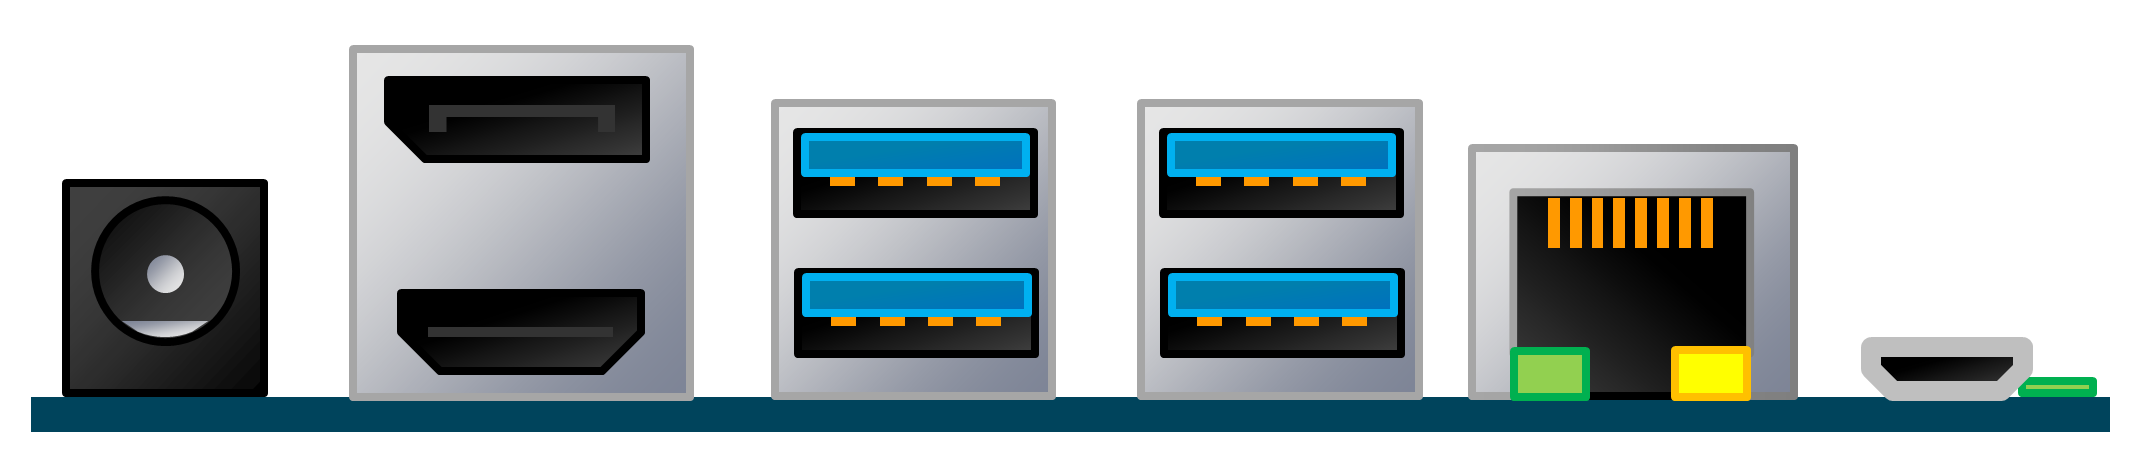
\includegraphics[scale=0.7]{Images/Jetson/JetsonNanoSide}};

\begin{figure}
	
	\begin{tikzpicture}
	% Platine
	\draw[greenblue,fill=greenblue] (0,-0.02) -- (12.35,-0.02) -- (12.35,-0.2) -- (0,-0.2) -- cycle;
	
	% 5V 
	\pgfmathsetmacro{\xmin}{0.2};
	\pgfmathsetmacro{\xmax}{1.4};
	\pgfmathsetmacro{\ymin}{0};
	\pgfmathsetmacro{\ymax}{1.33};
	\draw[black,  fill=grayleft!30!grayright, postaction={path fading=west,  fill=grayleft},  line width=1.0pt] 
	(\xmin, \ymin) -- (\xmin, \ymax) -- (\xmax,\ymax) -- (\xmax, \ymin) -- cycle;
	
	\draw[silver,fill=silver,domain=0:360] plot ({0.8+0.11*cos(\x)}, {0.75+0.11*sin(\x)});
	\draw[silver,fill=silver,domain=230:310] plot ({0.8+0.4*cos(\x)}, {0.75+0.4*sin(\x)});
	\draw[black,line width=1.0pt,domain=0:360] plot ({0.8+0.4*cos(\x)}, {0.75+0.4*sin(\x)});
	
	%Display Port und HDMI
	\pgfmathsetmacro{\xmin}{1.9};
	\pgfmathsetmacro{\xmax}{3.95};
	\pgfmathsetmacro{\ymin}{0};
	\pgfmathsetmacro{\ymax}{2.1};
	\draw[graycircle!50, fill=white!20!graylight, postaction={path fading=west,  fill=grayright!60}, line width=1.0pt
	] (\xmin, \ymin) -- (\xmin, \ymax) -- (\xmax,\ymax) -- (\xmax, \ymin) -- cycle;
	
	\draw[black,fill=grayleft!30!grayright, postaction={path fading=west,  fill=grayleft},
	line width=1.0pt]   (2.4, 0.17) -- (2.17,0.41) -- (2.17,0.64) -- (3.65,0.64) -- (3.65,0.41) -- (3.42,0.17) -- cycle;
	
	\pgfmathsetmacro{\xmin}{2.35};
	\pgfmathsetmacro{\xmax}{3.48};
	\pgfmathsetmacro{\ymin}{0.39};
	\pgfmathsetmacro{\ymax}{0.42};
	\draw[grayright,fill=grayright %graycircle!50, fill=white!20!graylight, postaction={path fading=west,  fill=grayright!60}, line width=1.0pt
	] (\xmin, \ymin) -- (\xmin, \ymax) -- (\xmax,\ymax) -- (\xmax, \ymin) -- cycle;
	
	\draw[black,fill=grayleft!30!grayright, postaction={path fading=west,  fill=grayleft},
	line width=1.0pt] (2.33,1.42) -- (2.1, 1.65) -- (2.1,1.92) -- (3.66,1.92) -- (3.66,1.42) -- cycle;
	\draw[grayright,fill=grayright] (2.47, 1.7) -- (2.47,1.6) -- (2.37, 1.6) -- (2.37,1.75) -- (3.47,1.75) -- (3.47,1.6) -- (3.37,1.6) -- (3.37,1.7) -- cycle;
	
	% USV 3.0 - 2 x 2 
	\foreach \j in {0,...,1}
	{
		\pgfmathsetmacro{\xmin}{4.4+2.15*\j};
		\pgfmathsetmacro{\xmax}{6.1+2.15*\j};
		\pgfmathsetmacro{\ymin}{0};
		\pgfmathsetmacro{\ymax}{1.8};
		\draw[graycircle!50, fill=white!20!graylight, postaction={path fading=west,  fill=grayright!60}, line width=1.0pt] (\xmin, \ymin) -- (\xmin, \ymax) -- (\xmax,\ymax) -- (\xmax, \ymin) -- cycle;
		
		\foreach \i in {0,...,1}
		{
			\pgfmathsetmacro{\xmin}{4.54+2.16*\j};
			\pgfmathsetmacro{\xmax}{5.96+2.16*\j};
			\pgfmathsetmacro{\ymin}{0.27+0.86*\i};
			\pgfmathsetmacro{\ymax}{0.78+0.86*\i};
			\draw[black,fill=grayleft!30!grayright, postaction={path fading=west,  fill=grayleft},
			line width=1.0pt] 
			(\xmin, \ymin) -- (\xmin, \ymax) -- (\xmax,\ymax) -- (\xmax, \ymin) -- cycle;
			
			\pgfmathsetmacro{\xmin}{4.6+2.16*\j};
			\pgfmathsetmacro{\xmax}{5.91+2.16*\j};
			\pgfmathsetmacro{\ymin}{0.52+0.82*\i};
			\pgfmathsetmacro{\ymax}{0.73+0.82*\i};
			\draw[cyan, fill=deepskyblue, line width=1.0pt] 
			(\xmin, \ymin) -- (\xmin, \ymax) -- (\xmax,\ymax) -- (\xmax, \ymin) -- cycle;
			
			\foreach \k in {0,...,3}
			{
				\pgfmathsetmacro{\xmin}{4.75+2.16*\j+0.29*\k};
				\pgfmathsetmacro{\xmax}{4.88+2.16*\j+0.29*\k};
				\pgfmathsetmacro{\ymin}{0.44+0.83*\i};
				\pgfmathsetmacro{\ymax}{0.48+0.83*\i};
				\draw[copper,fill=copper] (\xmin, \ymin) -- (\xmin, \ymax) -- (\xmax,\ymax) -- (\xmax, \ymin) -- cycle;
			}     
		}
	}
	
	% Ethernet
	\pgfmathsetmacro{\xmin}{8.55};
	\pgfmathsetmacro{\xmax}{10.5};
	\pgfmathsetmacro{\ymin}{0};
	\pgfmathsetmacro{\ymax}{1.5};
	\draw[graycircle!50, fill=white!20!graylight, postaction={path fading=west,  fill=grayright!60}, line width=1.0pt] (\xmin, \ymin) -- (\xmin, \ymax) -- (\xmax,\ymax) -- (\xmax, \ymin) -- cycle;
	
	\pgfmathsetmacro{\xmin}{8.8};
	\pgfmathsetmacro{\xmax}{10.2};
	\pgfmathsetmacro{\ymin}{0};
	\pgfmathsetmacro{\ymax}{1.25};
	\draw[black,  fill=grayleft!30!grayright, postaction={path fading=west,  fill=grayleft},  line width=1.0pt] (\xmin, \ymin) -- (\xmin, \ymax) -- (\xmax,\ymax) -- (\xmax, \ymin) -- cycle;
	
	\pgfmathsetmacro{\xmin}{8.8};
	\pgfmathsetmacro{\xmax}{9.25};
	\pgfmathsetmacro{\ymin}{0};
	\pgfmathsetmacro{\ymax}{0.3};
	\draw[darkpastelgreen,fill=greenyellow, line width=1.0pt] (\xmin, \ymin) -- (\xmin, \ymax) -- (\xmax,\ymax) -- (\xmax, \ymin) -- cycle;
	
	\pgfmathsetmacro{\xmin}{9.75};
	\pgfmathsetmacro{\xmax}{10.2};
	\pgfmathsetmacro{\ymin}{0};
	\pgfmathsetmacro{\ymax}{0.3};
	\draw[orange, fill=yellow, line width=1.0pt
	] (\xmin, \ymin) -- (\xmin, \ymax) -- (\xmax,\ymax) -- (\xmax, \ymin) -- cycle;
	
	\foreach \j in {0,...,7}
	{
		\pgfmathsetmacro{\xmin}{9     + 0.13*\j};
		\pgfmathsetmacro{\xmax}{9.068 + 0.13*\j};
		\pgfmathsetmacro{\ymin}{0.92};
		\pgfmathsetmacro{\ymax}{1.25};
		\draw[copper,fill=copper]   (\xmin, \ymin) -- (\xmin, \ymax) -- (\xmax,\ymax) -- (\xmax, \ymin) -- cycle;
	}
	
	\pgfmathsetmacro{\xmin}{11.8};
	\pgfmathsetmacro{\xmax}{12.25};
	\pgfmathsetmacro{\ymin}{0};
	\pgfmathsetmacro{\ymax}{0.1};
	\draw[darkpastelgreen,fill=greenyellow, line width=1.0pt] (\xmin, \ymin) -- (\xmin, \ymax) -- (\xmax,\ymax) -- (\xmax, \ymin) -- cycle;
	
	% HDMI
	\draw[silver,fill=silver, line width=1.0pt] (11.0, 0) -- (11.7,0) -- (11.9,0.17) -- (11.9, 0.35) -- (10.8,0.35) --  (10.8, 0.17) -- cycle;
	
	\draw[black,fill=black] (11.05, 0.125) -- (11.65,0.125) -- (11.75,0.22) -- (11.75, 0.25) -- (10.95,0.25) --  (10.95, 0.22) -- cycle;
	
	\node (P1) at (0.8,-0.6) {5V DC};
	\node (P2) at (3,-0.8) {\begin{tabular}{c} Display Port \\ HDMI \end{tabular}};
	\node (P2) at (5.2,-0.8) {\begin{tabular}{c} USB 3.0 \\ USB 3.0 \end{tabular}};
	\node (P2) at (7.4,-0.8) {\begin{tabular}{c} USB 3.0 \\ USB 3.0 \end{tabular}};
	\node (P2) at (9.5,-0.6) { GigEth };
	\node (P2) at (11.8,-1) {\begin{tabular}{c} Micro USB\\ PWR oder \\ USB Device\end{tabular}};
	\node (P2) at (12.9,-1.8) {PWR LED};
	
	\end{tikzpicture}
	\caption{Seitenansicht des Jetson Nanos} \label{JetonSeite}
\end{figure}	


\subsubsection{Externe Stromversorgung}

Der Jetson Nano benötigt eine externe Stromversorgung. Dazu muss ein Gleichstromnetzteil (5V\textdirectcurrent{} 2A) zur Verfügung stehen. Das Netzteil kann sowohl mit einem 5V-Netzteil über die 5V DC-Schnittstelle als auch Micro USB-Schnittstelle verbunden werden. Falls die 5V DC-Schnittstelle verwendet werden wird, ist ein Jumper erforderlich, der die beiden Pins von J48, die zwischen Kamera- und Netzteil-Anschluss liegen, überbrückt werden.  Der Durchmesser des Steckers ist 2,1mm.  Das Zentrum ist der positive Pol. Falls die Stromversorgung über die Micro USB-Schnittstelle erfolgt, muss der Jumper entfernt werden.



\subsubsection{HDMI und Display-Port}

Für den späteren Betrieb ist ein Monitor nicht notwendig, aber für die Inbetriebnahme 
und manche Anwendung doch sehr sinnvoll. Ein externer Monitor kann entweder an der 
HDMI-Schnittstelle oder am Display-Port angeschlossen werden. Dabei stehen verschiedene Auflösungen mit bis zu 4K zur Verfügung.

Es ist zu beachten, dass HDMI-auf-DVI-Adapter nicht unterstützt werden. Daher muss ein
Monitor eingesetzt werden, der HDMI- oder Display-Port-Eingang direkt unterstützt. In der Tabelle~\ref{Jetson:Aufloesungen}
sind die   möglichen Bildauflösungen gelistet, die unterstützt werden.

Falls in der Anwendung kein Monitor verwendet werden soll, so muss dies bei der Installation des Betriebssystem berücksichtigt werden.



\begin{table}
  \centering
  \begin{tabular}{cc}
    \textbf{Video Encode}  & \textbf{250MP/sec} \\   \hline
     H.264/H.265           & 1 $\times$  4K mit  30 f/sec \\
     H.264/H.265	       & 2 $\times$ 1080p mit 60 f/sec \\
     H.264/H.265	       & 4 $\times$ 1080p mit 30 f/sec \\
     H.264/H.265	       & 4 $\times$ 720p mit 60 f/sec  \\
     H.264/H.265	       & 9 $\times$ 720p mit 30 f/sec \\
  \end{tabular}
 \caption{Unterstützte Video-Encoding-Formate}\label{Jetson:Aufloesungen}
\end{table}



\subsubsection{$\mu$USB-Schnittstelle}


An der $\mu$USB-Schnittstelle kann ebenfalls ein Netzteil (5V\textdirectcurrent{} 2A) mit $\mu$USB-Ausgang
verwendet werden. $\mu$USB wurde gewählt, da preiswerte Netzteile mit dieser Schnittstelle einfach zu finden sind. Der maximale Stromverbrauch liegt bei 5W bis 10W. Es ist ein qualitativ hochwertiges Netzteil zu wählen. Falls ein ungeeignetes Netzteil genutzt wird, so startet der NVIDIA Jetson Nano nicht. Eine einfache Maßnahme ist ein Netzteil mit einem kürzeren Kabel zu verwenden, da diese zu einem geringeren Spannungsabfall führt.


%Als Beispiel für eine gute Stromversorgung hat NVIDIA das 5V 2,5A Schaltnetzteil von 
%\href{https://www.adafruit.com/product/1995}{Adafruit mit 20AWG MicroUSB-Kabel (GEO151UB-6025)} validiert.
%Es wurde speziell entwickelt, um häufige Probleme mit USB-Netzteilen zu lösen; 
%weitere Informationen finden Sie auf der verlinkten Produktseite.






\subsubsection{USB 3.0-Schnittstellen}

Der Jetson Nano verfügt über 4 USB 3.0-Schnittstellen. Der Stromverbrauch an einer USB-Schnittstelle ist limitiert auf 100mA. Falls das angeschlossene Gerät einen höheren Verbrauch hat, so muss dieses mit einer zusätzlichen Stromversorgung ausgestattet werden. In der Regel können die USB-Tastatur und die Maus angeschlossen werden. 

\subsubsection{Ethernet-Schnittstelle}

Mit Hilfe der Ethernet-Schnittstelle mit RJ45-Anschluss kann der Computer entweder direkt an das Internet angeschlossen werden oder mit einem anderen Rechner kommunizieren. Mit einem Patchkabel, das in den Router gesteckt wird, kann ein Gigabit-Ethernet verwendet werden kann. Es werden Ethernet-Verbindung auf der Basis von 10/100/1000BASE-T unterstützt.
Eine WiFi-Verbindung kann aber auch mit einem optionalen USB-Dongle für WLAN erreicht werden.


\subsubsection{Status-LED}

Die Status-LED zeigt an, ob der Jetson Nano mit Strom versorgt wird. Die Status-LED blinkt, falls das Netzteil nicht ausreichend oder zu viel Strom liefert.



\subsubsection{GPIOs}

Der Jetson Nano verfügt über eine Schnittstelle, über die Erweiterungen angeschlossen werden können.
An der Schnittstelle J41 werden 40 Anschlüsse nach außen geführt. Sie nennen sich \ac{gpio}. Damit können eigene Schaltungen angeschlossen werden und das Board  mit neuen Funktionen versehen werden. Hier können LEDs oder Motoren angeschlossen werden. 
Aber es stehen dort weitere interessante Schnittstellen vom Type SPI,  I$^2$C und  I$^2$S zur Verfügung.


\subsubsection{CSI-Anschluss für eine Kamera}

Die Jetson Nano ist zusätzlich mit einer Kamera-CSI-Anschluss ausgestattet. 
Die genaue Spezifikation ist \textbf{12 lanes ($3\times 4$ or $4 \times 2$) MIPI CSI-2 D-PHY 1.1 (1.5 Gb/s per pair)}. Falls geeignete Software eingesetzt wird, kann damit der Jetson Nano zur Bilderkennung eingesetzt werden.

Die \ac{csi} ist eine Spezifikation der Mobile Industry Processor Interface (MIPI) Alliance. Sie definiert eine Schnittstelle zwischen einer Kamera und einem Rechner. \cite{csi2:2018,csi2:2019} Die Spezifikation beschreibt sowohl den physikalischen Layer der Signalübertragung (D-PHY beziehungsweise C-PHY), als auch das darauf aufsetzende Protokoll zur Bilddatenübertragung. Zusätzlich spezifiziert sie ein Interface zur Kamerakonfiguration \ac{cci}, das ein Schnittstelle gemäß \ac{i2c} ist.


\subsubsection{microSD-Karte}


Der Jetson Nano verfügt über keine Festplatte, auf dem sich ein Betriebssystem befindet.
Daher muss es eine andere Möglichkeit geben, dieses zu speichern. Hierzu verwendet der Jetson Nano 
eine microSD-Karte. Die SD-Karte enthält das Betriebssystem, das gestartet werden soll, und die Anwendungsprogramme. Dementsprechend muss die SD-Karte gewählt sein. Sie sollte also  schnell und groß genug sein; das empfohlene Minimum ist eine 16GB UHS-1-Karte. Die Einschubmöglichkeit ist auf der Unterseite des Jetson Nanos. 




\subsection{Technische Daten}


%todo neu formulieren
\Mynote{Ausführen}

GPU

NVIDIA Maxwell architecture with 128 NVIDIA CUDA® cores


Prozessor

CPU

Quad-core ARM Cortex-A57 MPCore processor 


Memory


4 GB 64-bit LPDDR4, 1600MHz 25.6 GB/s 


Storage

16 GB eMMC 5.1 

In jedem Notebook sind eine Embedded Multi Media Card (eMMC), eine Festplatte oder eine SSD verbaut - oder eine Kombination daraus. Eine Embedded Multi Media Card ähnelt technisch einer SD-Karte und ist für Hersteller eine günstige Option, 16 bis 128 GByte fest verlöteten Speicherplatz anzubieten. EMMCs bieten wie SSDs geringe Zugriffszeiten, aber langsame sequenzielle Datentransferraten.



\ToDo{Werbung, Quellen fehlen, Siehe pdf-Dokumente bzgl. Raspberry Pi als Vorlage}
	
	

\section{Schnittstellen des Jetson Nanos}



\subsection{J41 Expansion Header Pinout - GPIO-Pins}

Der Jetson Nano kann auch mit anderen System kommunizieren. Für diese Kommunikation oder zur Steuerung externer Geräte kann es hilfreich sein, die Pins des J41 Headers steuern zu können. Die Pins erlauben verschiedene Arten der Kommunikation:

\begin{itemize}
  \item Serielle Kommunikation \ac{uart}
  \item Kommunikation  via \ac{i2c}
  \item \ac{spi}
  \item \ac{i2s}
  \item Direkte Kommunikation über \ac{gpio}
\end{itemize}    


%todo neu formulieren

Über die Kommunikation über \ac{gpio} werden binäre Signale zwischen zwei Systeme ausgetauscht. Es handelt sich also einfach um digitale Ein- und Ausgänge, die je nach Bedarf als Ein- oder Eingang definiert werden kann.

Standardmäßig sind alle Schnittstellensignal-Pins des Jetson Nano als \ac{gpio} konfiguriert. Die Pins 3, 5, 8, 9, 27 und 28 bilden hier Ausnahmen. 
Die Pins 3 und 5 und der Pins 27 und 28 sind für die beiden \ac{i2c}-Schnittstellen mit 
den Datenleitungen \ac{sda}  und die Leitung mit dem Taktsignal \ac{scl}.
Die Pins 8 und 10 sind für die Empfangsleitung (Rx) der einen und die Sendungsleitung (Tx) des \ac{uart} reserviert. \cite{JetsonUserManual:2020} 

Zur Nutzung der \ac{gpio} muss die GPIO-Bibliothek installiert  werden.\cite{GitHubGPIO:2020}.

\medskip

Das sogenannte Pinout des Jetson Nano ist in dieser Abbildung~\ref{Jetson:gpio} zu sehen.

%\begin{figure}
%  \centering
%
%   \GRAPHICS{0.5}{1.0}{Jetson/JetsonNano-pinout}
%   
%   \caption{Pin-Belegung J41 Expansion Header}\label{Jetson:gpio}
%
%\end{figure}
%

%Pi-Enthusiasten werden die Ähnlichkeit in der Pin-Benennung bemerken. Ich habe die Pins nach Farben gruppiert, aber ich weiß immer noch nicht, was all die sekundären Funktionen der Pins sind. 
%Die Linux(BCM)-Spalte enthält zwei Zahlen. Die Zahlen in Klammern sind Raspberry-Pi-ähnliche GPIO-Nummern, so dass die gleichen GPIO-Bibliotheken wie die Raspberry-Pi verwendet werden können. 
%Diese Tabelle wird aktualisiert, nachdem NVIDIA weitere Dokumentation veröffentlicht hat (ich glaube, es wird in einigen Wochen erwartet). 

%\GRAPHICSC{1.0}{1.0}{Images/Jetson/JetsonNanoPins}
%\GRAPHICSC{0.7}{1.0}{Images/Jetson/gpio-pinout}




%{\scriptsize
%	\begin{tabular}{|p{20mm}|p{15mm}|p{15mm}|>{\columncolor{blue}}c|>{\columncolor{blue}}c|p{15mm}|p{15mm}|p{15mm}|} % >{\columncolor{green}}	% 
%		Alt Function & Linux (BCM) & Name & Pin & Pin & Name & Linux (BCM) & Alt Function \\ \hline
%		\cellcolor{orange} DAP4\_DOUT & 78(21) & D21 & 40 & 39 &\GND & & \\
%		\cellcolor{orange} DAP4\_DIN  & 77(20) & D20 & 38 & 37 & D26 & 12(26) & SPI2\_MOSI \\
%		UART2\_CTS   & 51(16) &       D16 & 36 & 35 & D19        & 76(19) & DAP4\_FS \\
%		&        &      \GND & 34 & 33 & D13        & 38(13) & GPIO\_PE6 \\
%		LCD\_BL\_PWM & 168(12)&       D12 & 32 & 31 & D6         & 200(6) & GPIO\_PZ0 \\
%		&        &      \GND & 30 & 29 & D5         & 149(5) & CAM\_AF\_EN \\
%		&        & D1/ID\_SC & 28 & 27 & D0/ID\_SD  &        & \\         
%		SPI1\_CS1    & 20(7)  &        D7 & 26 & 25 &\GND        &        &  \\
%		SPI1\_CS0    & 19(8)  &        D8 & 24 & 23 & D11        & 18(11) & SP1\_SCK \\
%		SPI2\_MISO   & 13(25) &       D25 & 22 & 21 & D9         & 17(9)  & SP1\_MISO \\
%		&        &      \GND & 20 & 19 & D10        & 16(10) & SP1\_MOSI \\
%		SPI2\_CS0    & 15(24) &       D24 & 18 & 17 & 3.3V       &        & \\   
%		SPI2\_CS1    & 232(23)&       D23 & 16 & 15 & D22        & 194(22)& LCD\_TE \\   
%		&        &      \GND & 14 & 13 & D27        & 14(27) & SPI2\_SCK \\
%		DAP4\_SCLK   & 79(18) &       D18 & 12 & 11 & D17        & 50(17) & UART2\_RTS \\
%		&        & RXD/D15   & 10 &  9 &\GND        &        & \\
%		&        & TXD/D14   &  8 &  7 & D4         & 216(4) & AUDIO\_MCLK\\
%		&        &\GND       &  6 &  5 & SCL/D3     &        & \\
%		&        & 5V        &  4 &  3 & SDA/D2     &        & \\
%		&        & 5V        &  2 &  1 & 3.3V       &        & \\
%	\end{tabular}
%}
%


\begin{table}
    
    \centering	
    {\small%\scriptsize
        \begin{tabular}{|c|c|a|a|c|c|} \hline
            \rowcolor{white}	 Sysfs GPIO &   \begin{tabular}{c} \textcolor{white}{I}\\ \textcolor{white}{I}\end{tabular}    Name   \begin{tabular}{c} \textcolor{white}{I}\\ \textcolor{white}{I}\end{tabular}     & Pin & Pin & Name & Sysfs GPIO  \\ \hline
            gpio78 & \begin{tabular}{c}I2S\_4\_SDOUT \\ D21 \\ \end{tabular}  & 40 & 39 & \GND   &  \\ \hline
            gpio77 & \begin{tabular}{c}I2S\_4\_SDIN  \\ D20 \\ \end{tabular}  & 38 & 37 & \begin{tabular}{c}SPI\_2\_MOSI  \\ D26 \\ \end{tabular}  & gpio12  \\ \hline
            gpio51 & \begin{tabular}{c}UART\_2\_CTS  \\ D16 \\ \end{tabular}  & 36 & 35 & \begin{tabular}{c}I2S\_4\_LRCK  \\ D19 \\ \end{tabular}  & gpio76  \\ \hline
            & \GND                                                     & 34 & 33 & \begin{tabular}{c}GPIO\_PE6  \\ D13 \\ \end{tabular}     & gpio38  \\ \hline
            gpio168& \begin{tabular}{c}LCD\_BL\_PWM \\ D12 \\ \end{tabular}   & 32 & 31 & \begin{tabular}{c}GPIO\_PZ0  \\ D6 \\ \end{tabular}      & gpio200  \\ \hline
            & \GND                                                     & 30 & 29 & \begin{tabular}{c}CAM\_AF\_EN  \\ D5 \\ \end{tabular}    & gpio149  \\ \hline
            &\begin{tabular}{c}I2C\_1\_SCL\\D1/I2C Bus 0\\\end{tabular} & 28 & 27 & \begin{tabular}{c}I2C\_1\_SDA\\ D0/I2C Bus 0\\\end{tabular}  &         \\   \hline     
            gpio20 & \begin{tabular}{c}SPI\_1\_CS1\\ D7\\\end{tabular}    & 26 & 25 &\GND        &          \\ \hline
            gpio19 & \begin{tabular}{c}SPI\_1\_CS0\\ D8\\\end{tabular}    & 24 & 23 & \begin{tabular}{c}SPI\_1\_SCK\\ D11\\\end{tabular}            & gpio18  \\ \hline
            gpio13 & \begin{tabular}{c}SPI\_2\_MISO\\ D25\\\end{tabular}  & 22 & 21 & \begin{tabular}{c}SPI\_1\_MISO\\ D9\\\end{tabular}            & gpio17   \\  \hline
            &      \GND                                            & 20 & 19 & \begin{tabular}{c}SPI\_1\_MOSI\\ D10\\\end{tabular}           & gpio16  \\ \hline
            gpio15 & \begin{tabular}{c}SPI\_2\_CS0\\ D24\\\end{tabular}   & 18 & 17 & \Vd        &         \\  \hline 
            gpio232& \begin{tabular}{c}SPI\_2\_CS1\\ D23\\\end{tabular}   & 16 & 15 & \begin{tabular}{c}LCD\_TE\\ D22\\\end{tabular}       & gpio194 \\   \hline
            &      \GND                                            & 14 & 13 & \begin{tabular}{c}SPI\_2\_SCK\\ D27\\\end{tabular}   & gpio14  \\ \hline
            gpio79 & \begin{tabular}{c}I2S\_4\_SCLK\\ D18\\\end{tabular}  & 12 & 11 & \begin{tabular}{c}UART\_2\_RTS\\ D17\\\end{tabular}  & gpio50  \\ \hline
            & \begin{tabular}{c}UART\_2\_RX\\ /dev/ttyTHS1 - D15\\\end{tabular}  & 10 &  9 &\GND        &         \\ \hline
            & \begin{tabular}{c}UART\_2\_TX\\ /dev/ttyTHS1 - D14\\\end{tabular}  &  8 &  7 & \begin{tabular}{c}AUDIO\_MCLK\\ D4\\\end{tabular}        & gpio216 \\ \hline
            &\GND       &  6 &  5 & \begin{tabular}{c}I2C\_2\_SCL\\ I2C Bus 1 - D3\\\end{tabular}     &         \\ \hline
            & \Vf       &  4 &  3 & \begin{tabular}{c}I2C\_2\_SDA\\ I2C Bus 1 - D2\\\end{tabular}     &         \\ \hline
            & \Vf       &  2 &  1 & \Vd        &     \begin{tabular}{c} \textcolor{white}{I}\\ \textcolor{white}{I}\end{tabular}              \\ \hline
        \end{tabular}
    }
    
    \caption{Pinbelegung der GPIOs des Jetson Nanos} \label{Jetson:gpio}
\end{table}

%todo Nummern einfügen

\subsection{Serielle Schnittstelle J44 UART}

Der Jetson Nano verfügt über zwei Schnittstellen vom Typ \ac{uart}. Das serielle \ac{uart} kann für Anwendungen verwendet werden, die eine bidirektionale Kommunikation benötigen.



\begin{figure}
  \centering
  
  \begin{tikzpicture}[scale=1.4]
        %J44 Serial
        \pgfmathsetmacro{\xmin}{1.2};
        \pgfmathsetmacro{\xmax}{1.5};
        \pgfmathsetmacro{\ymin}{8.02};
        \pgfmathsetmacro{\ymax}{9.95};
        \draw[darkcyan,fill=greenblue,
        line width=1.6pt] (\xmin, \ymin) -- (\xmin, \ymax) -- (\xmax,\ymax) -- (\xmax, \ymin) -- cycle;
        
        \foreach \j in {0,...,0}
        {
            \foreach \i in {0,...,5}
            {
                \pgfmathsetmacro{\d}{0.05}
                \pgfmathsetmacro{\x}{1.35+0.312*\j};
                \pgfmathsetmacro{\y}{8.2+0.312*\i};
                \draw[yellow,fill=yellow] ({\x-\d}, {\y-\d} ) -- ({\x+\d}, {\y-\d}) -- ({\x+\d}, {\y+\d}) -- ({\x-\d}, {\y+\d}) -- cycle;
            }
        }
        \pgfmathsetmacro{\d}{0.05}
        \pgfmathsetmacro{\x}{1.35};
        \pgfmathsetmacro{\y}{8.2+0.312*0};
        \draw[yellow,thick,fill=fuchsia] ({\x-\d}, {\y-\d} ) -- ({\x+\d}, {\y-\d}) -- ({\x+\d}, {\y+\d}) -- ({\x-\d}, {\y+\d}) -- cycle;
        
        \node[right]  (P5) at (1.7,9.81) {CTS};
        \node[right]  (P5) at (1.7,9.48) {TXD};
        \node[right]  (P4) at (1.7,9.16) {TXD};
        \node[right]  (P3) at (1.7,8.82) {N/A};
        \node[right]  (P2) at (1.7,8.51) {RTS};
        \node[right]  (P1) at (1.7,8.16) {GND};
    \end{tikzpicture}
    
    \caption{J44 Serielle Schnittstelle - 3.3V 115200 Baud, 8N1} 
\end{figure}

\subsection{Schnittstelle J40 Buttons}


\begin{figure}
    \centering
    \begin{tikzpicture}[scale=1.4]
        % J40 Buttons
        \pgfmathsetmacro{\xmin}{0.17};
        \pgfmathsetmacro{\xmax}{0.82};
        \pgfmathsetmacro{\ymin}{7.7};
        \pgfmathsetmacro{\ymax}{9};
        \draw[darkcyan,fill=greenblue,
        line width=1.6pt] (\xmin, \ymin) -- (\xmin, \ymax) -- (\xmax,\ymax) -- (\xmax, \ymin) -- cycle;
        
        \foreach \j in {0,...,1}
        {
            \foreach \i in {0,...,3}
            {
                \pgfmathsetmacro{\d}{0.05}
                \pgfmathsetmacro{\x}{0.35+0.312*\j};
                \pgfmathsetmacro{\y}{7.87+0.312*\i};
                \draw[yellow,fill=yellow] ({\x-\d}, {\y-\d} ) -- ({\x+\d}, {\y-\d}) -- ({\x+\d}, {\y+\d}) -- ({\x-\d}, {\y+\d}) -- cycle;
            }
        }
        \pgfmathsetmacro{\d}{0.05}
        \pgfmathsetmacro{\x}{0.35+0.312};
        \pgfmathsetmacro{\y}{7.87+0.312*0};
        \draw[yellow,thick,fill=fuchsia] ({\x-\d}, {\y-\d} ) -- ({\x+\d}, {\y-\d}) -- ({\x+\d}, {\y+\d}) -- ({\x-\d}, {\y+\d}) -- cycle;
        
        \node[right]  (P4) at (1,8.85) {DIS (disable auto power-on)};
        \node[right]  (P3) at (1,8.5) {RST (system reset)};
        \node[right]  (P2) at (1,8.15) {FRC (board recovery mode))};
        \node[right]  (P1) at (1,7.8) {ON (power on) )};
        
    \end{tikzpicture}
    
    \caption{J40 Buttons}
\end{figure}  

\subsection{I\textsuperscript{2}C-Schnittstelle}

Der serielle Datenbus \ac{i2c} ermöglicht es dem Master-Gerät, Daten an ein Slave-Gerät zu senden oder Daten von einem Slave-Gerät anzufordern.

\subsection{I\textsuperscript{2}S-Schnittstelle}

\subsection{Serial Peripheral Interface (SPI)}

In der Standardkonfiguration hat der Jetson Nano keinen SPI-Port-Zugang. Allerdings kann dies an der SChnittstelle J41 Expansion Header konfiguriert werden.



\subsection{Power over Ethernet}

\subsection{Schnittstelle J15 zum Lüfter}


\begin{figure}
    \centering
    \begin{tikzpicture}[scale=1.4]
        % J15 5V Fan
        \pgfmathsetmacro{\xmin}{9.33};
        \pgfmathsetmacro{\xmax}{10.55};
        \pgfmathsetmacro{\ymin}{2.86};
        \pgfmathsetmacro{\ymax}{3.55};
        \draw[darkcyan,fill=greenblue,  line width=1.6pt] 
        (\xmin, \ymin) -- (\xmin, \ymax) -- (\xmax,\ymax) -- (\xmax, \ymin) -- cycle;
        
        \pgfmathsetmacro{\xmin}{9.8};
        \pgfmathsetmacro{\xmax}{10.45};
        \pgfmathsetmacro{\ymin}{3.35};
        \pgfmathsetmacro{\ymax}{3.55};
        \draw[darkcyan,
        line width=1.6pt] (\xmin, \ymin) -- (\xmin, \ymax) -- (\xmax,\ymax) -- (\xmax, \ymin) -- cycle;
        
        \foreach \j in {0,...,3}
        {
            \foreach \i in {0,...,0}
            {
                \pgfmathsetmacro{\d}{0.05}
                \pgfmathsetmacro{\x}{9.45+0.317*\j};
                \pgfmathsetmacro{\y}{3.18 +0.323*\i};
                \draw[blue,fill=yellow] ({\x-\d}, {\y-\d} ) -- ({\x+\d}, {\y-\d}) -- ({\x+\d}, {\y+\d}) -- ({\x-\d}, {\y+\d}) -- cycle;
            }
        }
        
        \draw[dotted] (9.45, 3.18) -- (9.45, 4.85) -- (9.6, 4.85);
        \node[right]  (P4) at (9.6,4.85) {PWM};
        \draw[dotted] (9.45+0.317, 3.18) -- (9.45+0.317, 4.5) -- (9.6+0.317, 4.5);
        \node[right]  (P3) at (9.6+0.317,4.5) {Tach};
        \draw[dotted] (9.45+0.317+0.317, 3.18) -- (9.45+0.317+0.317, 4.15) -- (9.6+0.317+0.317, 4.15);
        \node[right]  (P2) at (9.6+0.317+0.317,4.15) {5V};
        \draw[dotted] (9.45+0.317+0.317+0.317, 3.18) -- (9.45+0.317+0.317+0.317, 3.8) -- (9.6+0.317+0.317+0.317, 3.8);
        \node[right]  (P1) at (9.6+0.317+0.317+0.317,3.8) {GND};
        
        \pgfmathsetmacro{\d}{0.05}
        \pgfmathsetmacro{\x}{9.45+0.317*3};
        \pgfmathsetmacro{\y}{3.18};
        \draw[yellow,thick,fill=fuchsia] ({\x-\d}, {\y-\d} ) -- ({\x+\d}, {\y-\d}) -- ({\x+\d}, {\y+\d}) -- ({\x-\d}, {\y+\d}) -- cycle;
        
    \end{tikzpicture}
    
    \caption{J15 5V-Lüfter} 
\end{figure}


\section{Aufbau des Jetson Nanos}

\begin{itemize}
	\item Gehäuse
	\item WLAN
	\item Monitor
	\item Tastatur
\end{itemize}


\section{Betriebssystem JetPack für den Jetson Nano}

\subsection{Bescheibung des Betriebssystems}

NVIDIA stellt für den Jetson Nano eine eigenes Betriebssystem  \glqq JetPack\grqq{} zur Verfügung. Dieses Betriebsystem ist nicht nur für den Jetson Nano geeignet, sondern für die Jetson-Familie, bestehend aus  Jetson Nano, Jetson AGX Xavier und Jetson TX2.
Das Betriebssystem hat einen Linux-Kernel und besitzt das Debian Management Tool. Daher kann man auf der Grundlagen üblischer Linux-Kenntnisse mit dem System arbeiten. Insbesondere unterstützt es verschiedene Module für das Maschinelle Lernen:

\begin{itemize}
  \item CUDA, 
  \item TensorRT, 
  \item Computer Vision, 
  \item Deep Stream SDK.
\end{itemize}  

Dies ermöglicht eine Entwicklung für verschiedene Hardware-Systeme. Damit kann in Abhängigkeit der Anwendung die Leistung skaliert werden. \cite{Artamonov:2018,jetpack:2021} Die Abbildung~\ref{JetsonSDK} zeigt den Aufbau der Entwicklungsumgebung mit den genannten und weiteren Modulen. Die Einsatzmöglichkeiten der Module sind ebenfalls erwähnt.


%todo \Mynote{Erläuterung der Pakete}
% DeepStream SDK ermöglicht Entwicklern eine schnelle Erstellung und Bereitstellung effizienter Pipelines zur Videoanalyse auf Jetson-Basis. 

%\href{https://www.antratek.de/nvidia-jetson-xavier-nx-developer-kit?gclid=CjwKCAjwrcH3BRApEiwAxjdPTeWWscoBZWOLQgYzesZjl9OTE8WPs4v0Mrbv33llJ1hloT3Ncm85QRoCZ-UQAvD_BwE}{NVIDIA Jetson Xavier NX}
%\href{https://www.antratek.de/jetson-agx-xavier-developer-kit?gclid=CjwKCAjwrcH3BRApEiwAxjdPTXsHWj66yTy04tNZ29d2D_77W8crTU9Pty4WtZHzD5WPPst75SQRbBoCyN0QAvD_BwE}{NVIDIA Jetson AGX Xavier}
%\href{https://www.antratek.de/nvidia-jetson-tx2-development-kit}{NVIDIA Jetson TX2}

\medskip

\begin{figure}
	
	\GRAPHICSC{0.5}{1.0}{Jetson/JetsonNanoSDK}
	
	\caption{Jetson Nano SDK,  Quelle: Heise, 29.11.2019} \label{JetsonSDK}
\end{figure}


\subsection{Installation des Betriebssystems}



Das Betriebssystem muss auf einer microSD-Karte zur Verfügung gestellt werden. Eine Image-Datei findet sich auf der Website von NVIDIA\Mynote{Quelle}. Die Image-Datei wird von dort auf einen PC geladen. Mittels eines spezielle Programms, das das Dateisystem von JetPack, was mit dem Dateisystem von Linux übereinstimmt, berücksichtigt, auf die microSD-Karte geschrieben. Die microSD-Karte wird dann dem Jetson Nano zur Verfügung gestellt. Beim ersten Start kann das System konfiguriert werden. Dazu gehört unter anderem die Installation mit oder ohne grafischer Oberfläche. Die einzelnen Schritte werden nun erläutert.




\subsubsection{Schreiben des Betriebssystems auf die microSD-Karte}

Mit Hilfe eines Computers, der eine Internet-Verbindung besitzt, wird das Betriebssystem von der NVIDIA-Website geladen \cite{JetsonUserManual:2020, JetPackOS:2021}. Das Betriebssystem kann mit den üblichen Werkzeugen, z.B. Etcher, erhältlich auf der Website \textcolor{blue}{\url{https://www.balena.io/etcher/}}, auf eine microSD-Karte kopiert werden. \cite{JetsonGettingStarted:2019} 

Bei der Speicherkarte ist darauf zu achten, dass diese eine möglichst hohe Datenrate unterstützt, um die Ausführungsgeschwindigkeit des Betriebssystems nach Möglichkeit nicht zu verringern. Auf diese SD-Karte muss mit einem entsprechenden Tool, wie beispielsweise Balena Etcher\Mynote{Quelle}, das von der NVIDIA Website heruntergeladene NVIDIA JetPack Image für Jetson Nano entpackt werden. 


Zunächst muss die microSD-Karte formatiert werden:


\begin{enumerate}
  \item Windows:
	\begin{itemize}
		\item Formatieren Sie Ihre microSD-Karte mit dem SD-Speicherkarten-Formatierer der Firma SD Association \href{https://www.sdcard.org/downloads/formatter/}{[Link]}. Der SD-Karte-Formatierer muss installiert und gestartet werden.  Nach dem Start des Programms SD-Speicherkarten-Formatierer
		öffnet sich ein Dialog, siehe Abbildung~\ref{JetPack:SdFormatierer}.
		
		\begin{figure}
			\centering
			
     		\GRAPHICSC{0.5}{1.0}{Jetson/Jetson_Nano-Getting_Started-Windows-SD_Card_Formatter.png}
			\caption{Dialog zum Formatieren einer SD-Karte}\label{JetPack:SdFormatierer}
		\end{figure}
		
        Dann müssen folgende Schritte durchlaufen werden:

		  
		\begin{enumerate}  	  
			\item Zunächst muss die microSD-Karte in eine SD-Kartenlaufwerk eingelegt werden.
			\item Dann wird das richtig Kartenlaufwerk ausgewählt werden.
			\item Anschließend wird der Type \glqq Quick format\grqq{} gewählt.
			\item Das Feld \glqq Volume label\grqq{} darf nicht geändert werden.
			\item Danach kann durch Aktivierung des Knopfs \glqq Formatieren\grqq die Formatierung gestartet werden. Allerdings öffnet sich zunächst eine Warndialog, der mit dem Knopf \glqq Ja\grqq{} zu bestätigen ist.
		\end{enumerate}
		
		Nach der Formatierng der microSD-Karte kann man mit dem Programm Etcher die Image-Datei auf die microSD-Karte schreiben. Dzu sind folgende Schritte notwendig:
		
		\begin{enumerate}  	      	
			
			\item  Das Programm ist muss installiert und gestartet werden. Nach dem Start des Programms Etcher öffnet sich ein Dialog, siehe Abbildung~\ref{JetPack:SdFormatierer}.
			
		    \begin{figure}
		      \centering
  			  \GRAPHICSC{0.5}{1.0}{Jetson/Jetson_Nano-Getting_Started-Windows-Etcher.png}
			  \caption{Startdialog von Etcher}\label{JetPack:Etcher}
		    \end{figure}
			
			\item In diesem Startdialog ist zunächst der Knopf \glqq Bild auswählen\grqq{}. Dann kann die heruntergeladene Image-Datei aus.
			
			Falls die microSD-Karte nicht formatiert ist, meldet das Betriebssystem dies, siehe Abbildung~\ref{JetPack:NichtFormatiert}. Dann muss der Vorgang abgebrochen werden und die Karte muss zuerst formatiert werden.

            \begin{figure}
              \centering

              \GRAPHICSC{0.5}{1.0}{Jetson/Jetson_Nano-Getting_Started-Windows-Etcher_Cancel.png}
              
              \caption{Nicht formatierte Datei}\label{JetPack:NichtFormatiert}
            \end{figure}			
			
			\item Mit der Betätigung der Knopfes \glqq Flash!\grqq{} wird der Kopierprozess gestartet. Der Prozess dauert ca. 10 Minuten, falls eine USB 3-Schnittstelle verwendet wird. Während dieser Zeit schreibt Etcher die Image-Datei und validiert sie anschließend.
			\item  Nach Abschluss des Prozesses kann es vorkommen, dass Windows meldet, dass die microSD-Karte nicht gelesen werden kann, siehe Abbildung~\ref{JetPack:NichtLesen}. Diese Meldung ist zu ignorieren. Die microSD-Karte kann einfach aus dem Laufwerk entfernt werden. 
			
			\begin{figure}
				\centering
			
      			\GRAPHICSC{0.5}{1.0}{Jetson/Jetson_Nano-Getting_Started-Windows-SD_Card_Prompt.png}
	 
	            \caption{Windows-Meldung bei einer nicht formatierten microSD-Karte}\label{JetPack:NichtLesen}		
			\end{figure}
			
		\end{enumerate}
		
	\end{itemize}
\end{enumerate}  

Mit dem Entfernen der microSD-Karte aus dem Laufwerk ist Vorbereitung ihre Vorbereitung abgeschlossen. 

%todo https://developer.nvidia.com/embedded/learn/get-started-jetson-nano-devkit#setup	

\subsection{Einrichtung mit graphischer Oberfläche und erster Start}

Es liegt nun eine microSD-Karte vvor, die das Betriebssystem enthält. Jetzt kann der Jetson Nano vorbereit werden, um das Betriebssystem zu konfigurieren und zu nutzen. Es bestehen zwei grundlegende Möglichkeiten:

\begin{itemize}
    \item Verwendung mit grafischer Oberfläche
    \item Verwendung ohne grafischer Oberfläche
\end{itemize}

Vor der dem ersten Start muss diese Entscheidung getroffen werden. Eine Änderung kann später nicht mehr erfolgen. Dann besteht nur noch die Möglichkeit zum Wechsel, in dem das Betriebssystem neu installiert wird. Das heißt, es müssen auch alle Einstellungen wiederholt werden und die Software, die das Betriebssystem nicht bereit stellt, muss auch wieder hinzugefügt werden.

\bigskip

In diesem Abschnitt wird beschrieben, wie eine grafische Oberfläche konfiguriert wird.

\bigskip

Vor dem Einschalten des Jetson Nanos müssen einige Vorbereitungen getroffen werden. Zunächst muss ein Monitor über ein HDMI-Kabel, eine USB-Tastatur und eine USB-Maus angeschlossen werden. Der Jetson Nano steht bereit und auch ein geeignetes Netzteil. Allerdings darf das Netzteil noch nicht eingesteckt sein, da der Jetson Nano dann automatisch startet. Unter diesen Bedingungen wird die vorbereitete micorSD-Karte in den Jetson Nano eingesteckt. Jetzt kann das System eingeschaltet werden. Zunächst wird der Monitor eingeschaltet, dann wird das Netzteil an den Jetson Nano angeschlossen. Es leuchtet die grüne Leuchtdiode PWR LED auf und das System startet automatisch. Der Bootvorgang dauert einige Minuten. Beim Erststart muss dann das System konfiguriert werden. Die folgende Aufzählung listet die notwendigen Komponenten au.f.

\begin{itemize}
	\item Eine microSD-Karte mit dem Betriebssystem,
	\item Jetson Nano,
	\item \SI{5}{\volt}-Netzteil mit mindestens \SI{2.5}{\ampere} und mit Klinkenstecker,
	\item Ethernet-Kabel
	\item USB-Kabel mit microUSB-Stecker
	\item PC
	\item Ethernet-Anschluss
	\item Ethernet-Kabel
	\item Monitor mit HDMI-Anschluss oder Displayport; Adapter werden in der Regel  nicht unterstützt.
\end{itemize}


\subsubsection{Erster Start}

Während des ersten Bootvorgangs müssen einige Einstellungen vorgenommen werden:


\bigskip

Zuerst wird der Endbenutzer-Lizenzvertrag (End User License Agreement, EULA) von NVIDIA zur Jetson Nano Software angezeigt. Diesem Vertrag muss zugestimmt werden. Dann muss die Sprache eingestellt werden. Das Tastaturlayout kann ebenfalls gewählt werden. Dies sollte mit der angeschlossenen Tastatur übereinstimmen. Ebenfalls ist eine geeignete Zeitzone zu wählen. Dann müssen die Einstellungen vorgenommen werden, die bei der nächsten Anmeldung angefordert werden. Folgende Kennzeichnungen werden empfohlen:

	\begin{itemize}
		\item Einstellung des Namens: \textbf{MSR-Lab}
		\item Bezeichnung des Rechnernamens:\textbf{JetsonNanoMSRLab}
		\item Erstellung des Benutzernamens: \textbf{msrjetson}
		\item Festlegung des Kennwort: \textbf{MSR}
		\item Anmeldungsart: \textbf{Automatisch anmelden}
	\end{itemize}

Zuletzt muss die Größe der Partition angegeben werden. Für die Standardanwendung muss hier die maximale Größe angegeben werden. 




\subsubsection{Nach dem Anmelden}

Nach der erfolgreichen Konfiguration wird eine Willkommensmeldung, siehe~\ref{Jetson:Willkommen}, angezeigt. Das System kann nun genutzt werden.


\begin{figure}
  \centering
  
  \GRAPHICS{0.3}{1.0}{Jetson/Jetson_Nano-Getting_Started-Setup_Welcome_Screen.png}
 
  \caption{Willkommensmeldung nach dem ersten Start}\label{Jetson:Willkommen}
\end{figure}



\subsubsection{Deaktivierung der graphischen Oberfläche}


Um möglichst viel der Ressourcen des Jetson verwenden zu können, kann nach der Einrichtung der entsprechenden Gerätedaten (Nutzername, Gerätename, Passwort) die grafische Oberfläche über die Kommandozeile deaktiviert werden (\cref{src:nanogui}). Dies reduziert unter anderem die vom Betriebssystem beanspruchte Menge des Hauptspeichers, wodurch für spätere Anwendungen (wie TensorFlow) ein größerer Puffer vorhanden ist.

\begin{lstlisting}[language=MyBash, caption={Deaktivieren der graphischen Oberfläche des Jetson Nano}, label={src:nanogui}]
	$ sudo systemctl set-default multi-user.target
\end{lstlisting}

Falls eine \SI{16}{\giga\byte} Micro-SD verwendet wird, sollte ebenfalls darauf geachtet werden, dass nicht benötigte Anwendungen nach Möglichkeit vom System entfernt werden. Dies ist darauf zurückzuführen, dass der Installationsprozess von TensorFlow sehr viel Speicherplatz in Anspruch nimmt und dieser ansonsten nicht korrekt ausgeführt werden kann.

\begin{lstlisting}[language=MyBash, caption={Entfernen nicht benötigter Software vom JetPack Image}, label={src:nanoclean}, numbers=left]
	$ sudo apt update
	$ sudo apt remove -y libreoffice*
	$ sudo apt remove -y shotwell
	$ sudo apt remove -y thunderbird
	$ sudo apt remove -y chromium-browser
	$ sudo apt remove -y gnome-mahjongg
	$ sudo apt remove -y gnome-mines
	$ sudo apt remove -y gnome-sudoku
	$ sudo apt -y autoremove
	$ sudo apt -y autoclean 
\end{lstlisting}

Da \ac{pip} standardmäßig nicht auf dem System vorhanden ist, muss dieses mit den benötigten TensorFlow-Systemabhängigkeiten installiert werden (\cref{src:nanopip}).

\begin{lstlisting}[language=MyBash, caption={Installation von pip und TensorFlow-Abhängigkeiten auf Jetson Nano}, label={src:nanopip}, numbers=left]
	$ sudo apt install -y python3-pip
	$ sudo apt install -y libhdf5-serial-dev hdf5-tools libhdf5-dev zlib1g-dev zip libjpeg8-dev liblapack-dev libblas-dev gfortran
\end{lstlisting}

Im Anschluss kann nun TensorFlow mit \ac{pip} installiert werden. Um eine bestmögliche Kompabilität zu gewährleisten sollten hierfür die von NVIDIA zur Verfügung gestellten Paketquellen verwendet werden \cite{JetsonTensorFlow:2020}. Diese sind abhängig von der verwendeten JetPack-Version und installieren automatisch die aktuellste Paketversion, die mit dem System kompatibel ist. Falls die JetPack-Version unbekannt ist kann sie anhand der L4T-Version herausgefunden werden: \COMMAND{dpkg-query --show nvidia-l4t-core}. Als Beispiel: Version 32.4.3 entspricht JetPack 4.4; in der Index-URL muss also v44 eingetragen werden (\cref{src:nanotensorflow}). Je nach Geschwindigkeit der Micro-SD kann die Installation bis zu einer Stunde in Anspruch nehmen.

\begin{lstlisting}[language=MyBash, caption={Installation von TensorFlow auf Jetson Nano}, label={src:nanotensorflow}, numbers=left]
	$ pip3 install --upgrade cython # needed to install numpy
	$ pip3 install --no-cache-dir --extra-index-url https://developer.download.nvidia.com/compute/redist/jp/v44 tensorflow
\end{lstlisting}


\subsection{Einrichtung ohne graphischer Oberfläche}

Falls der Jetson Nano als Edge-Computer verwendet wird, besteht in der Regel nicht eine Möglichkeit, einen Monitor oder eine Tastatur anzuschließen. In diesem Fall muss das System so konfiguriert werden, dass keine Oberfläche installiert wird. Dies wird in diesem Abschnitt beschrieben.

Dazu müssen wieder Vorbereitungen getroffen werden. Folgende Teile sind bereit zu stellen:


\begin{itemize}
	\item Eine microSD-Karte mit dem Betriebssystem,
	\item Jetson Nano,
	\item \SI{5}{\volt}-Netzteil mit mindestens \SI{2.5}{\ampere} und mit Klinkenstecker,
	\item Ethernet-Kabel
	\item USB-Kabel mit microUSB-Stecker
	\item PC
	\item Ethernet-Anschluss
	\item Ethernet-Kabel
\end{itemize}


Da keine Oberfläche auf dem Jetson Nano installiert wird, muss er mit einem Rechner verbunden werden. Da Jetson Nano auch mit dem Internet verbunden sein muss, steht hierzu nur die Mikro USB-Schnittstelle zur Verfügung. Daher muss in diesem Fall ein Netzteil mit Klinkenstecker verwendet werden. Bevor das Netzteil angeschlossen wird, muss man den Jetson Nano mit dem Rechner über eine USB-Schnittstelle und mit dem Internet über ein Ethernet-Kabel verbunden werden. Ein Monitor darf nicht angeschlossen werden. Während des erstens Starts des Jetson Nanos wird dies geprüft; falls eine Monitor angeschlossen ist, so wird die grafische Oberfläche installiert. Nun kann die microSD-Karte in den Jetson Nano gesteckt werden. Jetzt kann der Jetson Nano eingeschaltet werden.


\section{Fernzugriff auf den Jetson Nano}

\subsubsection{Zugriff über Linux oder MacOS}

Nach dem Einschalten des Jetson Nano sucht man auf dem Linux- oder MacOS-Host in \SHELL{/dev} nach dem USB-Gerät. Beispielsweise ist das  \SHELL{tty.usbmodemFD133}. 
Mit diesem Gerät wird sich dann mit Hilfe des Terminal-Emulators \glqq screen\grqq{} verbunden:

\medskip

\SHELL{screen /dev/tty.usbmodemFD133 115200}

\subsubsection{Zugriff über Windows}

Unter Windows findet man die Schnittstelle des  Jetson Nano  als COM-Port. Mit dem Programm \glqq putty\grqq{} kann die Verbindung über die serielle Schnittstelle gestartet werden.

\subsubsection{Konfiguration des Jetson Nanos}

Bei erfolgreicher Verbindung werden mittels des Installationsassistenten \SHELL{oem-config} dann die erforderlichen Daten eingestellt. Wie bei der Installation mit grafischer Oberfläche wird zuerst der Endbenutzer-Lizenzvertrag (End User License Agreement, EULA) von NVIDIA zur Jetson Nano Software angezeigt. Diesem Vertrag muss zugestimmt werden. Dann muss die Sprache eingestellt werden. Das Tastaturlayout kann ebenfalls gewählt werden. Dies sollte mit der angeschlossenen Tastatur übereinstimmen. Ebenfalls ist eine geeignete Zeitzone zu wählen. Dann müssen die Einstellungen vorgenommen werden, die bei der nächsten Anmeldung angefordert werden. Folgende Kennzeichnungen werden empfohlen:

\begin{itemize}
    \item Einstellung des Namens: \textbf{MSR-Lab}
    \item Bezeichnung des Rechnernamens:\textbf{JetsonNanoMSRLab}
    \item Erstellung des Benutzernamens: \textbf{msrjetson}
    \item Festlegung des Kennwort: \textbf{MSR}
    \item Anmeldungsart: \textbf{Automatisch anmelden}
\end{itemize}


\bigskip

Danach steht der Jetson Nano zur Verfügung. Über ssh oder putty kann man sich dann mit dem Nano verbinden:

\medskip

\SHELL{ssh elmar@JetsonNanoMSRLab}

\medskip

%todo hier weiter neu formulieren.

%\url{https://medium.com/@heldenkombinat/getting-started-with-the-jetson-nano-37af65a07aab#f208}
\subsection{Einschalten und Aktivierung von Secure Shell}

\ac{ssh} ermöglicht den Zugriff auf den Jetson Nano, auch wenn dieser nicht mit einer Tastatur, Maus und Monitor
ausgestattet ist. Grundvoraussetzung ist die Verbindung des Jetson Nanos mit dem Netzwerk per Ethernet oder WLAN. 

\subsubsection{Installation von SSH}

Eine Installation von \ac{ssh} ist nicht notwendig, da es in der Distribution des Betriebssystems des Jetson Nanos enthalten ist. Dieser muss nur noch aktiviert werden.

%
%Aktuelle Versionen von Raspbian oder auch den meisten alternativen Linux-Distributionen kommen ab Werk mit einem SSH-Server. Dieser muss nur noch aktiviert werden. Falls eine ältere Version von Raspbian oder eine Distribution ohne vorinstallierten SSH-Server verwendet wird, kann dies schnell nachinstalliert werden. In einem Terminal am Raspberry Pi muss folgendes eingegeben werden:
%
%\medskip
%
%
%\SHELL{sudo apt-get install ssh}
%
%\medskip


\subsubsection{Aktivierung von SSH}


Zur Aktivierung von \ac{ssh} wird der \ac{ssh}-Server gestartet. Dies geschieht durch den folgenden Befehl:

\medskip

\SHELL{sudo /etc/init.d/ssh start}

\medskip

Da dies bei jder Verwendung von \ac{ssh} notwendig ist, wird dieser Vorgang automatisiert:

\medskip

\SHELL{sudo update-rc.d ssh defaults}

\medskip

Nach dieser Eingabe steht \ac{ssh} permanent, auch nach einem Neustart, zur Verfügung. Der Zugriff per \ac{ssh} auf den Jetson Nano ist dann immer möglich.

\bigskip

Eine weitere Möglichkeit  ist das Hinterlegen einer leeren Datei mit dem Namen \glqq ssh\grqq{} im Root-Verzeichnis. Falls die Datei vorhanden ist, ist \ac{ssh} beim nächsten Bootvorgang automatisch aktiviert.

\bigskip

Über die Systemeinstellungen kann der \ac{ssh}-Zugriff aktiviert werden. Dazu muss im Startmenü \menu[>]{Einstellungen > Konfiguration} der Konfigurationsdialog geöffnet werden, dort auf den Reiter \glqq Schnittstellen\grqq{} gewechselt und den Punkt \glqq SSH\grqq{} auf \glqq Aktiviert\grqq{} gesetzt werden. Nach der Bestätigung steht \ac{ssh} ebenfalls dauerhaft zur Verfügung. Zum Öffnen des Dialogs wird folgender Befehl verwendet:

\medskip

\SHELL{sudo raspi-config}

\medskip

Anschließend muss der Jetson Nano wieder neu gestartet werden:

\medskip

\SHELL{sudo reboot}


\subsubsection{Zugriff mittels Benutzernamem und IP-Adresse}

Für den \ac{ssh}-Zugriff muss der Benutzername und das Kennwort des Jetson Nanoss bekannt sein. Der Benutzername und das zugehörige Passwort wird bei der Konfiguration während des ersten Starts angegeben.
% Standardmäßig ist der Benutzername \glqq pi\grqq{} und das Passwort \glqq raspberry\grqq.
%Das Benutzerpasswort kann auf unterschiedliche Weise geändert werden, zum Beispiel im Konfigurationsmenü im Punkt \glqq Change password for the current user\grqq{} ändern. Auf der grafischen Benutzeroberfläche kann 
%dass Benutzerpasswort ebenfalls im Konfigurationsmenü geändert werden.


\bigskip

Damit \ac{ssh} verwendet werden kann, muss die IP-Adresse des Jetson Nanos bekannt sein. Mit dem Terminal-Befehl

\medskip

\SHELL{ifconfig}

\medskip

werden die aktuellen Netzwerkeinstellung inklusive der IP-Adresse ausgegeben.


%todo Testen!! und verbessern
%\medskip
%
%Wenn \ac{ssh} eingerichtet ist und danach die SD-Karte neu beschrieben und alles von Grund auf neu gestartet wird, erhält man eine Fehlermeldung.
%
%\medskip
%\SHELL{Remote Host Identification has changed}
%
%\medskip
%
%Mit dem Befehl
%
%\medskip

%\SHELL{ssh-keygen -f "/home/msr/.ssh/known\_hosts"{} -R "192.168.1.70"}
%
%wird das Problem behoben, falls der richtige Benutzer, hier msr, und die IP-Adresse des Jetson Nanos, hier 192.168.1.70,
%eingetragen wird.
%
%Für Windows-Benutzer ist beachten, die Nummer am Ende der Zeile der Fehlermeldung, die mit \SHELL{Offending ECDSA key in} beginnt. 
%Im obigen Windows-Beispiel ist diese Zahl 3. Schließlich muss die Datein \SHELL{known\_hosts} bearbeitet werden:
%
%\medskip
%
%\SHELL{notepad C:/Users/msr/.ssh/known\_hosts}
%
%\medskip
%
%wobei \SHELL{C:/Users/msr/.ssh/known\_hosts} durch den Pfad zu ersetzen ist, der in der Fehlermeldung angezeigt wird. 
%Die Zeile sollte die IP-Adresse Ihres Jetson enthalten.



%todo Testen!! und verbessern
\subsubsection{\ac{ssh}-Client unter Windows}


Seit 2017 besitzt Windows eine \ac{ssh}-Implementierung auf Basis von OpenSSH, die in der Kommandozeile PowerShell integriert ist. Zur Nutzung muss also über das Startmenü die PowerShell aufgerufen und folgender Befehl eingegeben werden:

\medskip

\SHELL{ssh benutzername@<IPAdresseDesJetsonNanos>}

\medskip

Bei der ersten Verbindung müssen  die \ac{ssh}-Schlüssel des Jetson Nanos mit \glqq yes\grqq{} bestätigt werden. Nach Eingabe des Benutzerpassworts kann der Fernzugriff durchgeführt werden.

%Der Vorgang ist ausführlicher im NVIDIA Jetson Linux Developer Guide beschrieben.


\subsection{Remote Desktop}




Wenn der Jetson Nano ohne Monitor, Tastatur und Maus betrieben werdne soll, dann sollte ein
Remote-Desktop-Access-Server namens \SHELL{xrdp} verwendet werden. Die Installation ist einfach:

\medskip

\SHELL{\$ sudo apt-get install xrdp}

\medskip

Nachdem die Installation abgeschlossen ist, muss der Jetson Nano neu gestartet werden. 
Sobald der Neustart abgeschlossen ist, kann durch den Befehl \SHELL{nmap}  auf dem PC überprüft werden, ob die Installation von 
\SHELL{xrdp} erfolgreich war:

\medskip

\SHELL{\$ nmap jetson}

\SHELL{Starting Nmap 7.70 ( https://nmap.org ) at 2019-04-13 01:39 BST}

\SHELL{Nmap scan report for jetson (192.168.1.118)}

\SHELL{Host is up (0.0025s latency).}

\SHELL{Not shown: 996 closed ports}

\SHELL{PORT     STATE SERVICE}

\SHELL{22/tcp   open  ssh}

\SHELL{111/tcp  open  rpcbind}

\SHELL{3389/tcp open  ms-wbt-server}

\SHELL{Nmap done: 1 IP address (1 host up) scanned in 1.25 seconds}

\SHELL{\$}

\medskip




%Wie Sie sehen können, da wir nicht eingeloggt sind, wurde unser VNC-Server heruntergefahren, aber der RDP-Server läuft, obwohl wir uns gerade auf dem Anmeldebildschirm des physischen Rechners befinden.
Obwohl Remote-Desktop-Protocol (RDP) ein proprietäres Protokoll ist, stellt Microsoft Viewer es für die meisten Plattformen kostenlos zur Verfügung. Dies muss installiert werden. Beim Windows-System muss im Programm Microsoft Remote Desktop
der Desktop hinzugefügt werden: \glqq Add Desktop\grqq

\medskip




Wenn die Einstellungen konfiguriert wurde, kann die Sitzung im Vollbildmodus durch eine vernünftige Auflösung 
für den resultierenden Fenster-Desktop eingestellt werden. 
%Klicken Sie auf "Speichern" und öffnen Sie dann den RDP-Desktop, indem Sie auf das Desktop-Symbol "Jetson Nano" klicken.

Wenn derPC über RDP mit dem Board verbunden ist, wird der Desktop etwas anders aussehen. Das liegt daran, dass  ein Standard-Ubuntu-Desktop angezeigt wird, auf dem Gnome läuft, und nicht den älteren Desktop im Unity-Stil, der bei L4T die Standardeinstellung ist. Das heißt, für den RDP wird ein eigener Desktop erstellt. Dieser
Desktop bleibt solange erhalten, bis sich der Benutzer abmeldet, das Schließen des RDP-Fenster führt nicht zum
Beenden des Desktops. Das heißt, beim nächsten Öffnen des RDP-Fensters steht der Desktop weitehrin zur Verfügung.


Allerdings ist zu beachten, dass man nicht gleichzeitig  auf dem physischen Desktop angemeldet sein kann  und einen RDP-Desktop öffnen.

Wenn der Jetson Nano über ein  drahtloses Netzwerk angesprochen wird, sollte in der Gnome-Anwendung 
unter \glqq Einstellungen\grqq{} im Menü auf der linken Seite \glqq Strom\grqq{} 
gewählt werden und sichergestellt sein, dass \glqq Wi-Fi ausschalten, um Strom zu sparen\grqq{} 
ausgeschaltet ist.


Nun können Monitor, Tastatur und Maus ausgesteckt werden, s werden nicht mehr benötigt.




\section{Installation von Software}

\subsection{Installation  pip}

Das Standard-Paketinstallationsprogramm \SHELL{pip} von Python ist auf dem Jetson Nano nicht vorinstalliert. Die Installation ist einfach:

\medskip

\SHELL{sudo apt install python3-pip}

\medskip



	

\subsection{Installation von cmake und git}

Es gibt jedoch eine umfangreiche erste Demonstrationsprojekt mit dem Titel \glqq Hello AI World\grqq, die von GitHub des Projekts herunterladen werden kann. Dazu müssen zunächst die Programme \SHELL{cmake} und \SHELL{git} installiert werden:

\medskip

\SHELL{\$ sudo apt-get install cmake}

\SHELL{\$ sudo apt-get install git}






\section{Installation der \ac{gpio}-Bibliothek}

Die Bibliothek zur Verwaltung und Nutzung der \ac{gpio}-Schnittstelle stellt NVIDIA in einem GitHub-Projekt zur Verfügung. Mit Hilfe des Befehls 


\medskip
\SHELL{\$ git clone https://github.com/NVIDIA/jetson-gpio}
\medskip

kann der Projekt auf den Jetson Nano kopiert werden. Anschließend kann die Bibliothek installiert werden. In dem Verzeichnis, wo sich die Datei \PYTHON{setup.py} des Projekts befindet, muss nun der Befehl



\medskip
\SHELL{\$ sudo python3 setup.py install}
\medskip

ausgeführt werden. Um mit der Bibliothek arbeiten zu können, muss man die Benutzerrechte besitzen. Dazu wird zunächst eine \ac{gpio}-Benutzergruppe mittels

\medskip
\SHELL{\$ sudo groupadd -f -r gpio} \newline
\medskip


angelegt. Dann kann man die entsprechenden Benutzerrechte setzen, indem ein Benutzer hinzugefügt wird:

\medskip
\SHELL{\$ sudo usermod -a -G gpio msrjetson}
\medskip

Das Programm udev verwaltet die Geräte. Diesem Programm muss man nun die Benutzerregeln mitteilen. Dazu wird die Datei 99-gpio.rules in das Verzeichnis rules.d kopiert.

\medskip
\SHELL{\$ sudo cp lib/python/Jetson/GPIO/99-gpio.rules /etc/udev/rules.d/}
\medskip

Diese Regel werden erst nach einem Neustart des Systems verwendet. Alternativ können die Regeln auch aktiv geladen werden:

\medskip
\SHELL{\$ sudo udevadm control -{}-reload-rules \&\& sudo udevadm trigger}
\medskip

Das GitHub-Projekt enthält auch Beispielprogramme, die sich in dem Ordner \SHELL{samples} befinden. Diese können zum Testen verwendet werden.  Ein Beispiel ist das Programm \PYTHON{simple\_out.py}. Es verwendet den BCM-Pin-Nummerierungsmodus des Raspberry Pis und gibt alle 2 Sekunden abwechselnd hohe und niedrige Werte an BCM-Pin 18, also Pin 12, aus. Damit kann eine LED zum Blinken gebracht werden kann. Der Aufruf erfolgt durch den folgenden Befehl:

\medskip
\SHELL{\$ python3 simple\_out.py}
\medskip

